\documentclass{ta-its}
\usepackage{hyperref} % Hyperlink pada dokumen
\usepackage{listings} % Kode sumber
\usepackage[verbose]{wrapfig}
\usepackage{etoolbox}
\usepackage{float}

\renewcommand{\lstlistingname}{Kode Sumber}
\renewcommand{\lstlistlistingname}{DAFTAR KODE SUMBER}


% \title{Judul Bahasa Indonesia}{Judul Bahasa Inggris}
\title{Rancang Bangun Sistem Penyeimbang Beban pada Klaster Server dengan Prioritas Berbasis Konten dan Kontrol Ketersediaan Layanan}{Design and Implementation of Load Balancing System with Content Priority and Availability Control}{KI141502} 

% \author{Nama Lengkap}{NRP}
\author{Bahrul Halimi}{5111100014}

% \supervisorOne{Nama Pembimbing Satu}{NIP}
% \supervisorTwo{Nama Pembimbing Dua}{NIP}
\supervisorOne{Royyana Muslim Ijtihadie, S.Kom, M.Kom, PhD}{197708242006041001}
\supervisorTwo{Baskoro Adi P, S.Kom, M.Kom}{198702182014041001}

% \degree{Nama Gelar}{Bidang Studi}{Program Studi}{Jurusan}{Jurusan (English)}{Fakultas}{Fakultas Singkatan}{Fakultas (English)}
\degree{Sarjana Komputer}{Arsitektur dan Jaringan Komputer}{S1}{Teknik Informatika}{Informatics}{Teknologi Informasi}{FTIf}{Information Technology}

% \time{bulan}{tahun}
\time{Desember}{2015}

\begin{document}
    \frontmatter % Halaman dengan penomoran romawi kecil
    \maketitle
    \legalityPaper % Lembar Pengesahan
    \begin{abstrak}
    	Aplikasi berbasis web semakin diminati untuk berbagai proses bisnis yang ada di lingkungan kita. Salah satu yang menjadi sorotan adalah penerimaan peserta didik baru yang dilaksanakan secara \textit{online}. Dengan adanya aplikasi ini pengguna akan dihadapkan pada dua jenis halaman yaitu halaman pengisian informasi untuk daftar dan halaman untuk menampilkan informasi. Tentu dengan pengaturan yang biasa, server akan melayani dua jenis halaman ini secara bersamaan. Kondisi ini akan mengakibatkan \textit{bottle neck} atau penumpukan permintaan. \\
	    Muncul gagasan untuk membagi beban kerja ke komputer lain agar setiap permintaan yang masuk dapat dilayani. Gagasan ini sudah biasa dilakukan dengan menggunakan Nginx sebagai balancer. Namun dengan beragamnya tipe permintaan pengguna, waktu yang dibutuhkan untuk melayani menjadi tidak stabil. \\
	    Gagasan lain muncul dengan adanya pembagian beban kerja berdasarkan konten yang diakses pengguna. Konten ini dapat diartikan sebagai dua jenis halaman sebelumnya. NodeJS akan bekerja sebagai balancer dan membaca setiap permintaan pengguna dan mengarahkan permintaan kepada \textit{worker} yang sesuai untuk setiap URL yang diakses pengguna. Dibantu dengan MongoDB sebagai basis data, NodeJS akan bekerja lebih konsisten terhadap data masuk ke sistem. \\
	    Hasil menunjukkan dengan NodeJS dan prioritas berbasis konten, waktu respon meningkat seiring dengan bertambahnya permintaan yang masuk. Namun dengan terfokusnya kerja \textit{worker} untuk melayani satu jenis halaman, membuat setiap permintaan dapat terlayani hingga permintaan selesai. \\
    	
    	\noindent \textbf{Kata-Kunci}: Load Balance, Prioritas Berbasis Konten, NodeJS, MongoDB.
	\end{abstrak}
	
	\cleardoublepage
   \begin{abstract}
	   	Web-based application become viral in our living society nowadays. One of those application is an on line application for student enrollment. In this kind of application user will access two type of page, the first one is a page with information from database or not and the second one is a page with an insert action to database. With a basic installation of server, server will serve this two type of page and make a bottle neck condition for high access. \\
	   	There is an idea to load balance every request to another computer, so every request can be handled. Usually, system administrator will use Nginx as a load balancer. But with multiple kind of request, response time to make every request handled, become unstable. \\ 
	   	Another idea appear, every request will be load balance with content based priority. Content is represented as two type of page before. Node JS will be used as load balancer system and read every header of request and redirect request to specific worker. With MongoDB as a database of system, NodeJS will work consistently for every data that come to the system. \\
	   	The result show that NodeJS and content-based priority will increase response time for increasing number of access from user. But the mechanism to make a worker focus on one type of page, make every request will be server well.
    	
    	
    	\noindent \textbf{Kata-Kunci}: Load Balance, Content Based Priority, NodeJS, MongoDB.
	\end{abstract}
	
    \chapter{Kata Pengantar}
	    \begin{figure}[h]
	    	\centering
	    	
\includegraphics[width=0.5\linewidth]{contoh_img/gambarBismillah}
	    \end{figure}

        Alhamdulillahirabbil’alamin, segala puji bagi Allah SWT, yang telah melimpahkan rahmat dan hidayah-Nya sehingga penulis dapat menyelesaikan Tugas Akhir yang berjudul \textbf{RANCANG BANGUN SISTEM PENYEIMBANG BEBAN PADA KLASTER SERVER DENGAN PRIORITAS BERBASIS KONTEN DAN KONTROL KETERSEDIAAN LAYANAN}. Pengerjaan Tugas Akhir ini merupakan suatu kesempatan yang sangat baik bagi penulis. Dengan pengerjaan Tugas Akhir ini, penulis bisa belajar lebih banyak untuk memperdalam dan meningkatkan apa yang telah didapatkan penulis selama menempuh perkuliahan di Teknik Informatika ITS. Dengan Tugas Akhir ini penulis juga dapat menghasilkan suatu implementasi dari apa yang telah penulis pelajari.
        Selesainya Tugas Akhir ini tidak lepas dari bantuan dan dukungan beberapa pihak. Sehingga pada kesempatan ini penulis mengucapkan syukur dan terima kasih kepada:
        \begin{enumerate}
        	\item Allah SWT atas anugerahnya yang tidak terkira kepada penulis dan Nabi Muhammad SAW.
        	\item Bapak, Ibu, Mbak Nova yang telah memberikan dukungan moral dan material serta doa yang tak terhingga untuk penulis. Serta selalu memberi semangat dan dorongan untuk segera menyelesaikan pengerjaan Tugas Akhir ini.
        	\item Bapak Royyana Muslim Ijtihadie, S.Kom, M.Kom, Ph.D. selaku pembimbing I yang telah membantu, membimbing, dan memotivasi penulis mulai dari pengerjaan proposal hingga terselesaikannya Tugas Akhir ini.
        	\item Bapak Baskoro Adi P, S.Kom, M.Kom selaku pembimbing II yang juga telah membantu, membimbing, dan memotivasi penulis mulai dari pengerjaan proposal hingga terselesaikannya Tugas Akhir ini.
        	\item Ibu Dr. Eng. Nanik Suciati, S.Kom., M.Kom., selaku Kepala Jurusan Teknik Informatika ITS pada masa pengerjaan Tugas Akhir, Bapak Darlis Herumurti, S.Kom., M.Kom., selaku Kepala Jurusan Teknik Informatika ITS saat ini, Bapak Radityo Anggoro, S.Kom., M.Sc., selaku koordinator TA, dan segenap dosen Teknik Informatika yang telah memberikan ilmu dan pengalamannya.
        	\item Teman-teman Laboratorium AJK, samihd, romen, vivi, harum, dimas, thiar, agus, surya, pur, eva, nisa, uul, wicak, zaza, daniel, nindy, rizma, asbun, oing, fatih, syukron yang selalu menghibur dan mendukung penulis dalam pengerjaan Tugas Akhir ini.
        	\item Yang selalu memberikan semangat, memasakkan makanan ketika penulis sakit, memarahi ketika penulis lupa dengan Tugas Akhir, dan memberikan hiburan ketika penulis terhenti pada pengerjaan Tugas Akhir.
        	\item Teman-teman Kidnapper PARESMAPA angkatan 21 yang selalu mendukung penulis untuk tidak segera lulus.
        	\item Teman-teman di Dinas Pendidikan Kota Surabaya yang memberikan semangat untuk segera menyelesaikan Tugas Akhir.
        	\item Serta semua pihak yang telah turut membantu penulis dalam menyelesaikan Tugas Akhir ini.
        \end{enumerate}
        
        Penulis menyadari bahwa Tugas Akhir ini masih memiliki banyak kekurangan. Sehingga dengan kerendahan hati, penulis mengharapkan kritik dan saran dari pembaca untuk perbaikan ke depannya.
        
        \hfill Surabaya, Desember 2015 \\ \\
        
        
        \hfill Bahrul Halimi

        \cleardoublepage % Mengisi penanda halaman genap yang kosong

    \tableofcontents % Daftar isi
    \listoftables % Daftar tabel
    \listoffigures % Daftar figur/gambar
    \lstlistoflistings % Daftar kode sumber

\mainmatter % Halaman utama, dengan judul BAB X, nomor halaman penomoran arab
    \chapter{PENDAHULUAN}
        Pada bab ini akan dipaparkan mengenai garis besar Tugas Akhir yang meliputi latar belakang, tujuan, rumusan dam batasan permasalahan, metodologi pembuatan Tugas Akhir, dan sistematika penulisan.

        \section{Latar Belakang}
            Semakin berkembangnya internet di masyarakat membuat penggunaan aplikasi berbasis web semakin diminati. Pengguna aplikasi berbasis web ini dapat dijumpai diberbagai aktivitas harian masyarakat, diantaranya bank \emph{online}, \emph{e-commerce}, reservasi tempat secara \emph{online}, bahkan pendaftaran peserta didik baru secara \emph{online} (PPDB Surabaya). Hal ini membuat penyedia layanan aplikasi berbasis web harus menyediakan servis yang layak sehingga aplikasi tetap berjalan dengan baik walaupun pengguna semakin bertambah.\\
			\indent Terjadinya \emph{bottleneck} (penumpukan permintaan) menjadi tantangan tersendiri ketika pengembang tidak memperhatikan sumber dayanya dan berujung pada gagalnya permintaan pengguna \cite{paperAlgoritma}. Muncul gagasan awal dengan penggunaan kelompok server yang akan menangani permintaan ini. Kelompok server ini akan secara bergantian melayani setiap permintaan terhadap aplikasi berbasis web ini. Dengan adanya tugas bergantian ini dibutuhkan sebuah komputer yang bertugas membagi beban kerja kelompok server. Komputer ini biasa disebut pembagi muat atau \emph{load balancer}. Sistem kerja dari \emph{load balancer} ini menggunakan sebuah algoritma yang sudah ditanam untuk kemudian digunakan untuk memilih komputer mana yang harus melayani permintaan pengguna. Pada titik ini, banyak penyedia layanan web memutuskan menggunakan Nginx sebagai \textit{load balancer}, dengan alasan kemampuannya menangani banyak permintaan, dibangingkan Apache \cite{quoraNginx}\cite{aosaNginx}. \\
			\indent Di sisi lain sebuah aplikasi berbasis web memiliki dua jenis halaman yang mungkin di akses. Yang pertama adalah halaman berisi informasi, baik hasil \emph{query} basis data maupun tidak, selanjutnya disebut halaman informasi dan yang kedua adalah halaman yang digunakan untuk mengirimkan data ke server, dalam hal ini berupa form pengisian informasi, selanjutnya disebut halaman daftar. \\
			\indent Dua jenis halaman ini memiliki kebutuhan yang berbeda. Untuk halaman informasi, pengguna mengharapkan akses yang cepat sedangkan untuk halaman daftar, pengguna mengharapkan data yang dimasukkan dapat diproses dengan aman. Padahal di dalam penggunaan mekanisme sebelumnya dan dengan teknologi yang ada, \emph{load balancer} tidak dapat memisahkan dua jenis permintaan ini. Mekanisme yang ada sebelumnya hanya memisahkan banyak permintaan sesuai dengan ketersediaan server melayani pengguna. Padahal ketika proses pemasukkan data di dalam halaman daftar, seharusnya bisa digunakan untuk melayani permintaan pada halaman informasi. \\
			\indent Muncullah gagasan lain mengenai pengelompokkan permintaan berdasarkan konten yang diinginkan oleh pengguna. Pengelompokkan ini didasarkan pada dua halaman sebelumnya, yakni halaman informasi dan halaman daftar. Tujuannya untuk mengatur penggunaan sumber daya yang digunakan. Dua kelompok server terpisah akan melayani masing-masing permintaan yang berbeda. Dengan permintaan satu tipe dalam satu kelompok server, membuat kerja server menjadi lebih terpusat dan mengurangi beban yang besar. \\
			\indent Berbeda dengan yang terjadi saat ini, sebuah server atau bahkan dalam sebuah kelompok server, harus melayani berbagai bentuk permintaan dari pengguna, sehingga menyebabkan beban kerja server meningkat. Bahkan waktu dalam penyelesaian suatu permintaan tidak dapat diukur dalam satuan waktu yang sama karena berbedanya bentuk permintaan pengguna. \\
			\indent Sementara itu di dalam kelompok server yang bekerja bergantian melayani permintaan, ada kalanya sebuah server mengalami gangguan dan sama sekali tidak dapat melayani setiap permintaan pengguna. Padahal setiap permintaan yang ada masih diteruskan oleh load balancer pada server tersebut. Tidak adanya mekanisme untuk memindahkan permintaan dari server mati ke server yang masih aktif membuat akses ke sebuah web menjadi tidak maksimal. \\
			\indent Oleh karena itu dibangunlah sistem ini. Dengan adanya sistem load balancing menggunakan algoritma berbasis konten yang memisahkan antara halaman informasi dan halaman daftar diharapkan dapat meningkatkan jumlah pengguna suatu halaman web dengan banyaknya bentuk permintaan dari pengguna. Sistem ini juga akan dibandingkan dengan sistem yang sudah berjalan sebelumnya dengan studi kasus sistem Pendaftaran Peserta Didik Baru Surabaya tahun 2015 dengan Nginx sebagai \textit{load balancer}.

            
        \section{Rumusan Masalah}
			Berikut beberapa hal yang menjadi rumusan masalah dalam tugas akhir ini:
			\begin{enumerate}
			\item Bagaimana membagi beban kerja server berdasarkan konten permintaan pengguna ?
			\item Bagaimana menentukan pengelompokkan server berdasarkan konten permintaan pengguna ?
			\item Bagaimana meningkatkan jumlah pengakses pada halaman informasi dengan terpisahnya akses antara halaman informasi dan halaman daftar ?
			\item Bagaimana menjaga pengguna tetap dilayani kelompok ser-ver yang tersedia hingga permintaan selesai ?
			\item Bagaimana perbandingan penggunaan CPU dan memori antara sistem baru dan yang sudah berjalan sebelumnya ?
			\end{enumerate}

        \section{Batasan Masalah}
			Dari permasalahan yang telah diuraikan di atas, terdapat beberapa batasan masalah pada tugas akhir ini, yaitu:
			\begin{enumerate}
			\item Konten permintaan pengguna dilihat dari URL yang diakses.
			\item Pendefinisian kelompok konten permintaan pengguna dilakukan manual oleh manusia.
			\item Sistem pembagi beban kerja diimplementasikan untuk aplikasi berbasis web.
			\item Kelompok server yang bekerja dibedakan dengan besar memori yang digunakan.
			\item Sistem yang akan dibandingkan adalah sistem untuk PPDB Surabaya tahun 2015 dengan Nginx sebagai \textit{load balancer}.
			\end{enumerate}

        \section{Tujuan}
			Tugas akhir dibuat dengan beberapa tujuan. Berikut beberapa tujuan dari pembuatan tugas akhir:
			\begin{enumerate}
			\item Mampu mengategorikan permintaan pengguna terhadap suatu web berdasarkan halaman yang diakses pengguna.
			\item Mampu melayani banyaknya permintaan pengguna dengan mengandalkan pengelompokan komputer.
			\item Mampu meningkatkan jumlah pengakses yang dilayani dengan berhasil oleh aplikasi dibandingkan dengan akses tanpa pemisahan jenis halaman yang diakses.
			\end{enumerate}

        \section{Manfaat}
			Dengan dibangunnya \emph{load balancer} ini diharapkan jumlah pengakses yang mampu dilayani oleh kelompok server untuk halaman informasi menjadi lebih banyak dibandingkan dengan penggunaan algoritma dan teknologi \emph{load balancing} yang sudah ada.

   \chapter{LANDASAN TEORI}
        \section{Prioritas Berbasis Konten}
			Munculnya mekanisme ini didasarkan pada beberapa jenis permintaan pengguna yang mengakses suatu halaman web. Sebuah server melayani berbagai jenis permintaan akan memberikan waktu balasan yang beragam pula. Hal ini akan meningkatkan beban kerja server. \\
			\indent Dengan adanya pemisahan permintaan pengguna berdasarkan konten, kelompok server akan melayani setiap permintaan yang memang ditujukan untuknya server tersebut. Bentuk permintaan akan selalu sama sehingga waktu untuk melayani permintaan menjadi sama dan lebih terkontrol. Beban kerja server akan lebih ringan dengan adanya pembagian beban berdasarkan algoritma ini \cite{paperAlgoritma}.

        \section{Node JS}
			Merupakan sebuah platform yang dibangun di atas Chrome's JavaScript runtime dengan teknologi V8 yang mendukung proses server yang bersifat long-running. Tidak seperti platform modern yang mengandalkan multithreading, NodeJS memilih menggunakan asynchronous I/O eventing. Karena inilah NodeJS mampu bekerja dengan konsumsi memori rendah \cite{webNodeJS}\cite{useNodeJS}.
			
			Teknologi yang tidak memanfaatkan multi-thread ini memudahkan pengembang yang terkadang kesulitan mengatur sumberdaya yang digunakan thread. Karena tidak mungkin ada sumberdaya yang terkunci karena thread yang berjalan. Akhirnya banyak yang memanfaatkan kemampuan dasar NodeJS sebagai web server.
			
			\begin{figure}[h] % h = pasti berada di bawah teks yang ada di atas
				\centering
				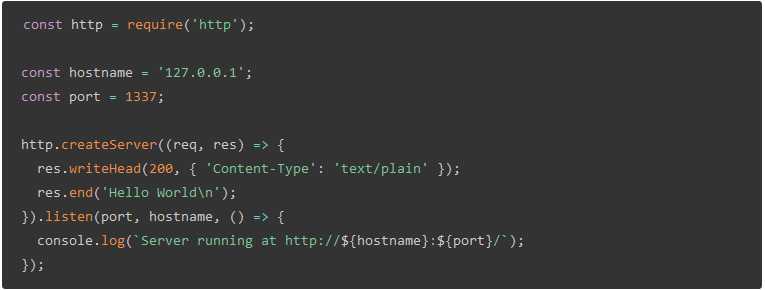
\includegraphics[width=\linewidth]{contoh_img/contoh_nodejs}
				\caption{Contoh Penggunaan NodeJS sebagai Web Server}
				\label{contohNodeJS}
			\end{figure}
			
			
			Dengan adanya callback untuk setiap penggunaan fungsi, memungkinkan setiap pemanggilan fungsi yang tidak menghasilkan apapun, NodeJS akan \textit{sleep}.

        \section{Angular JS}
			Angular JS membantu dalam pembangunan halaman HTML menjadi lebih dinamis. Merupakan sebuah kumpulan alat bantu yang mampu bekerja baik dengan pustaka lainnya. Setiap fitur dapat dimodifikasi sesuai dengan kebutuhan aplikasi. Menjadi salah satu kerangka kerja yang memfasilitasi pembangunan aplikasi kompleks yang terorganisir dan mudah dirawat. Angular JS lebih dikenal pada kemampuannya melayani sebuah situs web yang menggunakan halaman tunggal untuk penyajian data yang beragam \cite{clientSideWeb}\cite{angularJS}.
			
			\begin{figure}[h] % h = pasti berada di bawah teks yang ada di atas
				\centering
				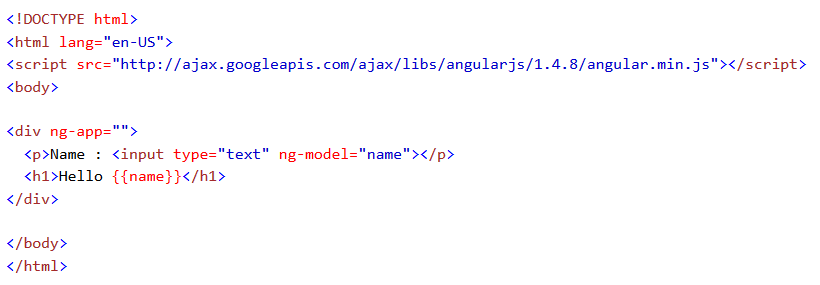
\includegraphics[width=\linewidth]{contoh_img/contoh_angular}
				\caption{Contoh Penggunaan Angular JS pada Halaman Sederhana}
				\label{contohAngularJS}
			\end{figure}

			Dengan menggunakan berkas JavaScript Angular yang didapatkan dari CDN (\textit{Content Delivery Network}) atau media lain, pengembang dapat dengan mudah menggunakan fitur yang ditawarkan Angular JS.
			
		\section{MongoDB}
			Merupakan salah satu NoSQL (Not only SQL) terkenal yang dirancang untuk mengelola polimorfik, obyek, dan struktur data yang terus berkembang. MongoDB adalah basis data open-source yang memungkinan mengubah skema dengan cepat sementara fungsi yang diharapkan dari basis data tradisional masih berjalan \cite{selfDescription}\cite{mongoDB}.
			
			\begin{figure}[h] % h = pasti berada di bawah teks yang ada di atas
				\centering
				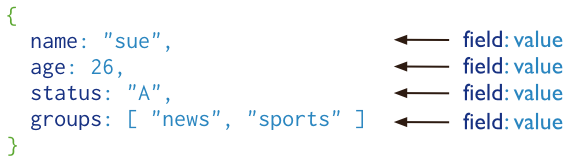
\includegraphics[width=\linewidth]{contoh_img/contoh_mongodb}
				\caption{Contoh Bentuk Penyimpanan Data MongoDB}
				\label{contohMongoDB}
			\end{figure}
			
			Model penyimpanan yang menyerupai JSON membuat pengguna dapat dengan mudah mengakses dan mengubah data yang ada. Karena penyimpanannya yang menyerupai JSON, membuat struktur penyimpanan dapat berubah sewaktu-waktu tanpa mengubah konfigurasi sebelumnya.
		
		\section{Apache JMeter}
			Menjadi salah satu alat bantu untuk melakukan tes muat dan mengukur performa aplikasi, salah satunya berbasis web. Mampu melakukan pengujian pada berbagai protokol diantaranya Web, FTP, basis data, Mail (SMTP, POP3, IMAP), serta MongoDB \cite{JMeter}.
			
			\begin{figure}[h] % h = pasti berada di bawah teks yang ada di atas
				\centering
				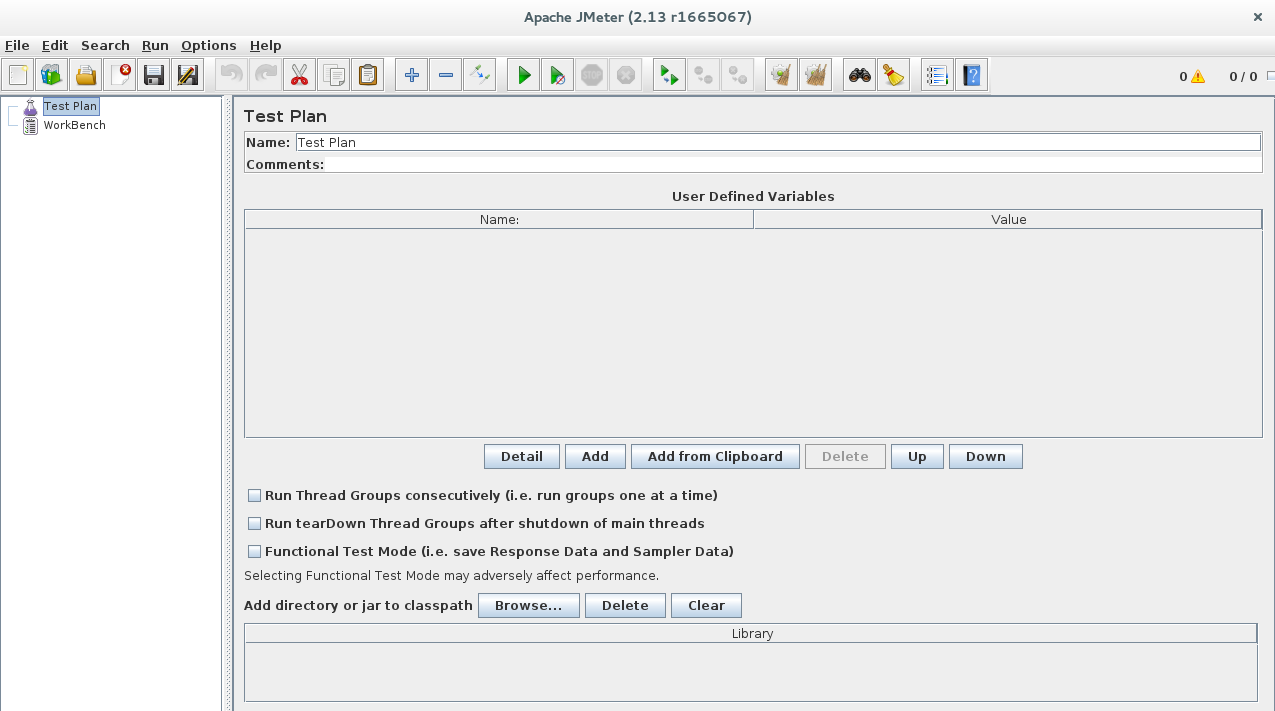
\includegraphics[width=\linewidth]{contoh_img/contoh_jmeter}
				\caption{Contoh Antar Muka Apache JMeter}
				\label{contohJMeter}
			\end{figure}
			
			Apache JMeter berbasis Java. Cara kerjanya yang menyerupai sebuah browser, karena desain awal memang ditujukan untuk menguji aplikasi berbasis web, mampu mengakses halaman website yang memiliki sumber daya statis maupun dinamis. Namun ada beberapa fitur browser yang tidak ditiru oleh Apache JMeter.


    \chapter{DESAIN DAN PERANCANGAN}
	    Pada bab ini dibahas mengenai analisis dan perancangan sistem.
	    
	    \section{Kasus Penggunaan}
		    Terdapat dua aktor dengan masing-masing tiga aktivitas dalam sistem yang digambarkan pada Gambar \ref{gambarDiagramKasusPenggunaan}.
		    
		    \begin{figure}[h] % h = pasti berada di bawah teks yang ada di atas
		    	\centering
		    	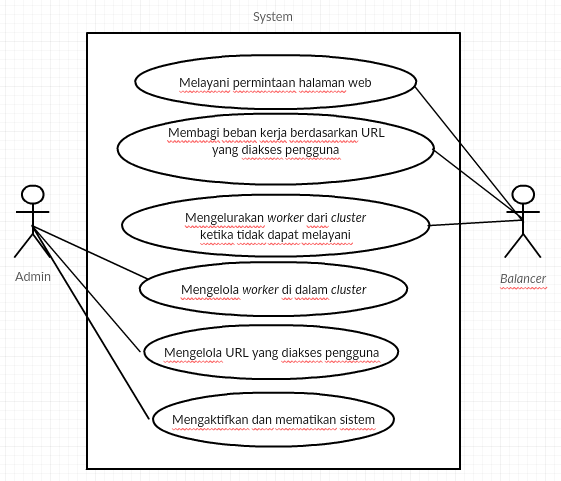
\includegraphics[width=\linewidth]{contoh_img/usecase}
		    	\caption{Digram Kasus Penggunaan}
		    	\label{gambarDiagramKasusPenggunaan}
		    \end{figure}
		    
		    Digram kasus penggunaan pada Gambar \ref{gambarDiagramKasusPenggunaan} dideskripsikan masing-masing pada Tabel \ref{tabelKodeKasusPenggunaan}.
		    \begin{ltabulary}{|L|L|L|} % L = Rata kiri untuk setiap kolom, | = garis batas vertikal.
		    	
		    	% Kepala tabel, berulang di setiap halaman
		    	\caption{Daftar Kode Kasus Penggunaan} \label{tabelKodeKasusPenggunaan} \\
		    	\hline
		    	\textbf{Kode Kasus Penggunaan} & \textbf{Nama Kasus Penggunaan} & \textbf{Keterangan} \\ \hline
		    	
		    	\endhead
		    	\endfoot
		    	\endlastfoot
		    	
		    	% Isi Tabel
		    	UC-0001 & Melayani permintaan halaman web & Setiap permintaan halaman web akan mengarah ke sistem dan \textit{balancer} akan melayani dengan cara meneruskan permintaan ke \textit{worker} dan mengeruskan balasan ke pengguna \\ \hline
		    	UC-0002 & Membagi beban kerja berdasarkan URL yang diakses pengguna & Dibelakang sistem terdapat beberapa \textit{worker} yang bekerja melayani permintaan terusan dari sistem, di sini lah \textit{balancer} membagi beban kerja tersebut \\ \hline
		    	UC-0003 & Mengeluarkan \textit{worker} dari klaster ketika tidak dapat melayani & Jika terdapat \textit{worker} yang tidak dapat melayani permintaan, \textit{balancer} akan mengeluarkan sementara dari tugas melayani hingga \textit{worker} mampu memberikan layanan \\ \hline
		    	UC-0004 & Mengelola \textit{worker} di dalam klaster & Admin dapat menambahkan dan mengurangi \textit{worker} di dalam daftar klaster \\ \hline
		    	UC-0005 & Mengelola URL yang diakses pengguna & Admin dapat menambahkan dan mengurangi daftar URL ke dalam sistem \\ \hline
		    	UC-0006 & Mengaktifkan dan mematikan sistem & Admin memiliki kendali atas aktif dan tidaknya sistem \\ \hline
		    	
		    \end{ltabulary}
		    
		\section{Arsitektur Sistem}
			Pada sub-bab ini, dibahas mengenai tahap analisis dan kebutuhan bisnis dan desain dari sistem yang akan dibangun.
	    
		    \subsection{Desain Umum Sistem}
			    Sistem load balancing yang akan dibangun menggunakan teknologi Node JS dengan JavaScript sebagai bahasa pemrograman. Sistem ini akan berjalan pada port 80 dan menjadi target utama ketika pengguna akan menggunakan aplikasi berbasis web yang dikembangkan dengan menggunakan load balancer ini. Akan terdapat beberapa komputer pembantu, selanjutnya disebut \textit{worker}, yang menerima perintah untuk melayani permintaan halaman website dari load balancer. \textit{Worker} akan digolongkan menjadi dua cluster untuk melayani permintaan sesuai dengan URL yang diakses pengguna. Di sinilah algoritma berbasis konten diterapkan. Secara visual, desain sistem secara umum digambarkan pada Gambar \ref{gambarSistem}.
			    
			    \begin{figure}[h] % h = pasti berada di bawah teks yang ada di atas
			    	\centering
			    	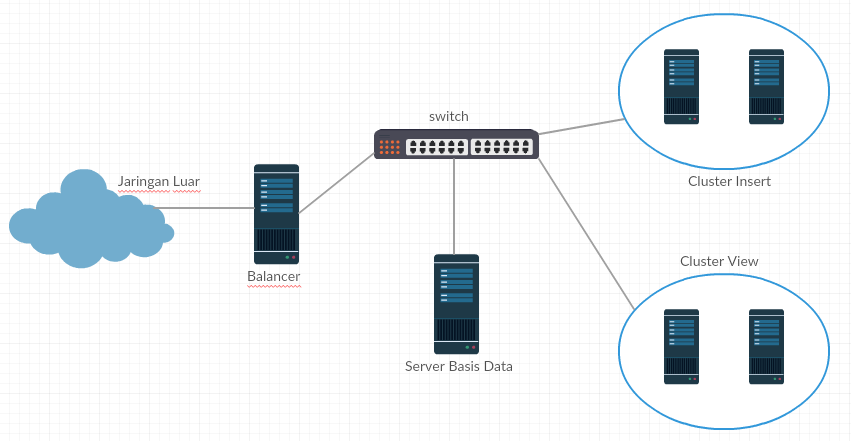
\includegraphics[width=\linewidth]{contoh_img/sistem}
			    	\caption{Desain Sistem Secara Umum}
			    	\label{gambarSistem}
			    \end{figure}
			    
			    Load balancer memiliki daftar \textit{worker} dan URL yang akan digunakan dalam operasional load balancing. Daftar ini disimpan dalam MongoDB agar daftar yang dimiliki konsiste. MongoDB menyimpan data dalam bentuk JSON sehingga koneksi untuk mendapatkan daftar ini cepat.
			    
			    Untuk memudahkan administrator sistem dalam mengkonfigurasikan \textit{worker} dan menambahkan daftar URL yang ada, disediakan sebuah halaman admin yang berjalan pada port 3000. Selain dengan halaman admin ini, administrator sistem sudah dibantu untuk mengeluarkan \textit{worker} yang tidak aktif dari pekerjaannya dalam proses load balancing oleh sistem secara otomatis dalam rentang waktu tertentu.
			    
			    
			    
			
			\subsection{Desain Balancer}
			    \textit{Balancer} berperan penting dalam sistem. Setiap permintaan yang masuk ke dalam sistem akan diolah oleh balancer dan dikembalikan ke pengguna setelah mendapat balasan dari \textit{worker}. Ada beberapa aplikasi yang sudah menyediakan fitur \textit{balancing}, namun dalam Tugas Akhir ini digunakan NodeJS dan MongoDB untuk membangun fitur \textit{balancing}. Diagram arsitektur Balancer tertera pada Gambar \ref{gambarArsitekturBalancer} dan diagram proses pengguna mengakses halaman web tertera pada Gambar \ref{gambarKerjaBalancer}. 
			    
			    \begin{figure}[] % h = pasti berada di bawah teks yang ada di atas
			    	\centering
			    	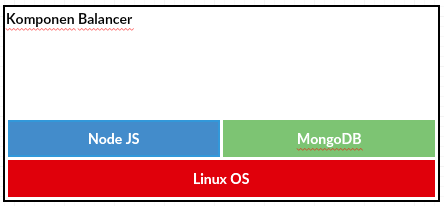
\includegraphics[width=\linewidth]{contoh_img/kompbalancer}
			    	\caption{Desain Arsitektur Balancer}
			    	\label{gambarArsitekturBalancer}
			    \end{figure}
			    
			    NodeJS akan menyediakan servis web yang akan menangkap setiap permintaan pengguna. Sebelum diteruskan ke \textit{worker}, \textit{balancer} akan membaca data tentang klaster di dalam MongoDB. Data di dalam database berupa \textit{worker} yang siap melayani permintaan berdasarkan URL yang ada. Setelah \textit{balancer} mendapatkan satu \textit{worker} yang siap, permintaan diteruskan untuk mendapatkan balasan yang sesuai. Setelah mendapatkan balasan dari \textit{worker}, balasan dikembalisan ke pengguna.
			    
			    Setiap aktivitas yang terjadi di \textit{balancer} akan dicatat dan disimpan pada MongoDB. Semua data yang dibutuhkan \textit{balancer} tersimpan pada MongoDB dan disajikan pada halaman admin.
			    			    
			    \begin{figure}[] % h = pasti berada di bawah teks yang ada di atas
			    	\centering
			    	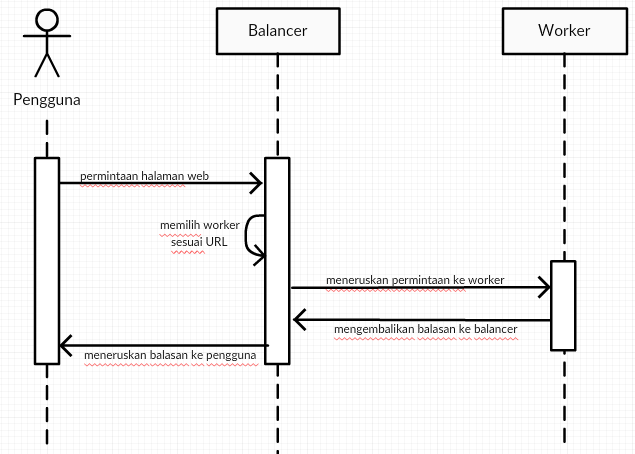
\includegraphics[width=\linewidth]{contoh_img/kerjabalancer}
			    	\caption{Diagram Interaksi antara Pengguna, Balancer dan Worker}
			    	\label{gambarKerjaBalancer}
			    \end{figure}
			
			\subsection{Desain Worker}
				Worker bekerja sebagai pemberi layanan. Menunggu permintaan yang diteruskan dari balancer dan mengembalikan lagi ke balancer. Aplikasi berbasis web yang akan diakses pengguna dijalankan pada \textit{worker}. Diagram arsitektur \textit{worker} tertera pada Gambar \ref{gambarArsitekturWorker}
				
				\begin{figure}[] % h = pasti berada di bawah teks yang ada di atas
					\centering
					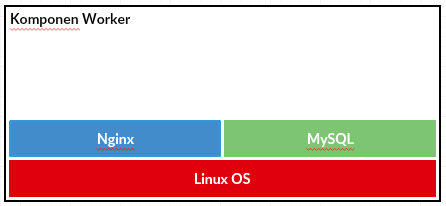
\includegraphics[width=\linewidth]{contoh_img/kompworker}
					\caption{Diagram Arsitektur Worker}
					\label{gambarArsitekturWorker}
				\end{figure}
				
				Di dalam sistem yang dibangun, peran \textit{worker} sudah digambarkan pada diagram proses yang tertera pada Gambar \ref{gambarKerjaBalancer}. Pengguna tidak dapat mengakses \textit{worker} secara langsung. Semua akses harus melalui \textit{balancer}. Walaupun sebenarnya semua aplikasi berada pada \textit{worker}.
			
			\subsection{Desain Halaman Admin}
				Halaman ini hanya akan diakses oleh administrator sistem. Adanya halaman ini ditujukan untuk memudahkan admin dalam mengelola cluster dan mengelola URL yang tersimpan di dalam basis data. Digram arsitektur halaman admin tertera pada Gambar \ref{gambarArsitekturWeb}.
				
				\begin{figure}[] % h = pasti berada di bawah teks yang ada di atas
					\centering
					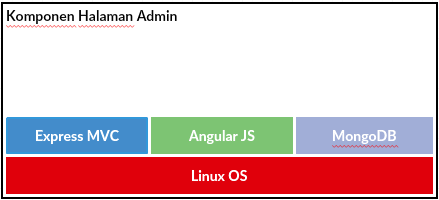
\includegraphics[width=\linewidth]{contoh_img/kompweb}
					\caption{Diagram Arsitektur Halaman Admin}
					\label{gambarArsitekturWeb}
				\end{figure}
				
				Express JS berperan dalam menangkap setiap rute yang diminta admin. Sementara Angular JS digunakan untuk menampilkan data sesuai dengan rute yang diminta admin. MongoDB yang digunakan dalam halaman admin sama dengan MongoDB yang digunakan oleh \textit{balancer}. Daftar rute yang dapat diakses admin tertera pada Tabel \ref{tabelRuteHalamanAdmin}.
				
				\begin{longtable}{|p{0.05\textwidth}|p{0.15\textwidth}|p{0.2\textwidth}|p{0.4\textwidth}|} % L = Rata kiri untuk setiap kolom, | = garis batas vertikal.
					
					% Kepala tabel, berulang di setiap halaman
					\caption{Rute pada Halaman Admin} \label{tabelRuteHalamanAdmin} \\
					\hline
					\textbf{No} & \textbf{Rute} & \textbf{Metode} & \textbf{Aksi} \\ \hline
					
					\endhead
					\endfoot
					\endlastfoot
					
					% Isi Tabel
					1 & / & GET, POST & Menampilkan status balancer dan operasi mengaktifkan/mematikan \textit{balancer}\\ \hline
					2 & /cluster & GET, POST & Mengelola \textit{worker} di dalam klaster \\ \hline
					3 & /path & GET, POST & Mengelola rute pada aplikasi sesuai dengan klaster \\ \hline

				\end{longtable}
				
			\subsection{Desain Server Basis Data}
				Dalam menjalankan sebuah aplikasi yang menuntut kemampuan akses hingga banyak pengguna, banyak pengembang yang memisahkan antara server aplikasi dan server basis data. Aplikasi yang berjalan dalam server ini hanya MySQL sebagai basis data seperti yang tertera pada \ref{gambarArsitekturDB}.
			    
				\begin{figure}[h] % h = pasti berada di bawah teks yang ada di atas
					\centering
					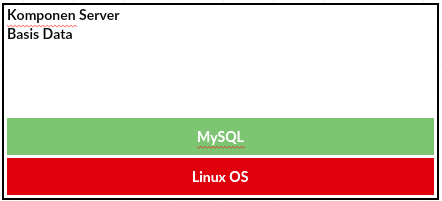
\includegraphics[width=\linewidth]{contoh_img/kompdb}
					\caption{Diagram Arsitektur Server Basis Data}
					\label{gambarArsitekturDB}
				\end{figure}


% vAB 4 BAB 4 BAB 4 BAB 4 BAB 4 BAB 4 BAB 4 BAB 4 BAB 4 BAB 4 BAB 4 BAB 4 BAB 4 BAB 4 BAB 4 BAB 4 BAB 4 BAB 4 BAB 4 BAB 4 BAB 4 BAB 4 BAB 4 BAB 4 BAB 4 BAB 4 BAB 4 BAB 4 BAB 4 BAB 4 BAB 4 BAB 4 BAB 4 BAB 4 BAB 4 BAB 4 BAB 4 BAB 4 BAB 4 BAB 4 BAB 4 BAB 4 BAB 4 BAB 4 BAB 4 BAB 4 BAB 4 BAB 4 BAB 4 BAB 4 BAB 4 BAB 4 BAB 4 BAB 4 BAB 4 BAB 4 BAB 4 BAB 4 BAB 4 BAB 4 BAB 4 BAB 4 BAB 4 BAB 4 BAB 4 BAB 4 BAB 4 BAB 4 BAB 4 BAB 4 BAB 4 BAB 4 BAB 4 BAB 4 BAB 4 BAB 4 BAB 4 BAB 4 BAB 4 BAB 4 BAB 4 BAB 4 BAB 4 BAB 4
		         
		         
	\chapter{Implementasi}
        Bab ini membahas implementasi sistem Load Balancing secara rinci. Pembahasan dilakukan secara rinci untuk setiap komponen yang ada yaitu: Balancer, Worker, Halaman Admin, dan Server Basis Data.
        
        \section{Lingkungan Implementasi}
	        Lingkungan implementasi dan pengembangan dilakukan menggunakan komputer dengan spesifikasi Intel(R) Core(TM) i3-2120 CPU @ 3.30GHz dengan memori 8 GB di Laboratorium Arsitektur dan Jaringan Komputer, Teknik Informatika ITS. Perangkat lunak yang digunakan dalam pengembangan adalah sebagai berikut :
	        \begin{itemize}
	        	\item Sistem Operasi Linux Ubuntu Server 14.04.01 LTS
	        	\item Desktop xfce4
	        	\item Editor teks vim
	        	\item Editor teks Sublime Text 2
	        	\item git versi 1.9.1 untuk pengolahan versi program
	        	\item NodeJS versi 4.2.3 untuk pengembangan aplikasi
	        	\item MongoDB versi 3.2.0 untuk basis data
	        	\item Express versi 4.13.1 untuk web server halaman admin
	        	\item Angular JS versi 1.5.0-beta.2 untuk pengolahan data pada halaman admin
	        	\item Nginx versi 1.4.6 untuk implementasi sistem PPDB Surabaya tahun 2015
	        	\item Paket \LaTeX untuk pembuatan buku tugas akhir
	        	\item Peramban \textit{web} Mozilla Firefox
	        \end{itemize}
	        
		\section{Rincian Implementasi Balancer}
		
			\textit{Balancer} dibangun dengan menggunakan Node JS, MongoDB dan beberapa paket yang diinstall secara terpisah. Paket-paket ini diinstall dengan menggunakan npm (\texttt{https://www.npmjs.com/}) yang memang digunakan sebagai \textit{command line} oleh Node JS. Pada sub bab ini akan dijelaskan implementasi balancer hingga \textit{balancer} siap digunakan.
			
			\subsection{Instalasi Paket untuk NodeJS}
			Seperti yang sudah dijelaskan sebelumnya, instalasi paket yang dibutuhkan menggunakan npm. Cara kerja npm ini hanya mengunduh paket untuk kebutuhan sistem, hanya saja beberapa paket bisa diinstall pada sistem operasi dan dapat digunakan pada \textit{command line}. 
			Untuk mengunduh paket yang dibutuhkan secara bersamaan, digunakan perintah \texttt{npm install}. Perintah ini akan membaca file \texttt{package.json} yang berisi daftar paket yang akan digunakan. Isi \texttt{package.json} untuk Tugas Akhir ini seperti pada Kode Sumber \ref{packageJson}

			\begin{lstlisting}[frame=single,tabsize=2,breaklines,caption={Isi Package.Json},label=packageJson]
{
	"name": "tugasakhir",
	"version": "1.0.0",
	"description": "Tugas Akhir ini berisi tentang load balancer dengan node JS",
	"dependencies": {
		"body-parser": "~1.13.2",
		"cookie-parser": "~1.3.5",
		"debug": "~2.2.0",
		"express": "~4.13.1",
		"express-session": "^1.7.6",
		"express-socket.io-session": "^1.3.1",
		"hbs": "~3.1.0",
		"helmet": "^0.10.0",
		"http-proxy": "^1.12.0",
		"moment": "~2.x.x",
		"mongoose": "^4.3.1",
		"morgan": "~1.6.1",
		"mysql": "~2.x.x",
		"net-ping": "^1.1.12",
		"node-sass-middleware": "0.8.0",
		"request": "^2.67.0",
		"serve-favicon": "~2.3.0",
		"socket.io": "~1.x.x"
	},
	"devDependencies": {},
	"scripts": {
		"test": "echo \"Error: no test specified\" && exit 1"
	},
	"repository": {
		"type": "git",
		"url": "git+https://github.com/bahrulhalimi/tugasakhir.git"
	},
	"keywords": [
		"balancer",
		"TA",
		"nodeJS"
	],
	"author": "Bahrul Halimi",
	"license": "ISC",
	"bugs": {
		"url": "https://github.com/bahrulhalimi/tugasakhir/issues"
	},
	"homepage": "https://github.com/bahrulhalimi/tugasakhir#readme"
}

				
			\end{lstlisting}
			
				Selain paket yang diinstall melalui perintah \texttt{npm install}, ada beberapa paket yang harus di install ke dalam sistem untuk bisa dipanggil melalui \textit{command line}. Salah satu paket yang digunakan dalam Tugas Akhir ini adalah \texttt{forever}. Paket ini harus di install ke komputer, sehingga dapat digunakan melalui \textit{command line}. Untuk menginstallnya digunakan perintah \texttt{sudo npm install forever -g}.
        
	        \subsection{Koneksi ke Basis Data}
		        Pada Tugas Akhir ini digunakan paket yang membantu untuk menghubungkan aplikasi dengan basis data yaitu paket \texttt{mongoose}. Untuk dapat terhubung dengan basis data, digunakan perintah \texttt{mongoose.connect('mongodb://127.0.0.1/tugasakhir')}
		        
		        Karena basis data yang digunakan MongoDB dan bersifat NoSQL, maka struktur tabel menjadi tidak wajib di deklarasikan di awal. Untuk selanjutnya dibuat model untuk mendeklarasikan setiap koneksi ke basis data, sesuai dengan tabel yang digunakan. Dalam MongoDB istilah tabel menjadi koleksi (\textit{collection}). Terdapat empat koleksi yang dibuat yaitu:
		        
		        \begin{itemize}
		        	\item aktivitas\_model, digunakan untuk mencatat setiap permintaan ke sistem.
		        	\item clusterinsert\_model, digunakan untuk mencatat daftar \textit{worker} di dalam \textit{cluster insert}.
		        	\item clusterview\_model, digunakan untuk mencatat daftar \textit{worker} di dalam \textit{cluster view}.
		        	\item path\_model, digunakan untuk mencatat daftar URL dan digolongkan ke dalam dua jenis, yaitu insert dan view.
		        	\item setting\_model, digunakan untuk mencatat konfigurasi \textit{balancer} terkait \textit{worker} default dan waktu untuk melakukan pengecekan terhadap \textit{worker} yang tidak aktif.
		        \end{itemize}
		        
		        Kode program untuk setiap model tertera pada lampiran.
			
			\subsection{Implementasi Balancer}
				Mekanisme prioritas berbasis konten diterapkan untuk menjalankan balancer. Mekanisme ini hanya akan memilih \textit{worker} sesuai dengan klaster yang aktif dan siap melayani permintaan. Daftar \textit{worker} yang dapat digunakan didapatkan dari basis data yang diakses dengan menggunakan model yang sudah di bahas pada sub-bab sebelumnya. Selanjutnya setiap permintaan akan dilempar ke \textit{worker} terpilih dan dilayani hingga permintaan selesai. Daftar paket yang akan digunakan tertera pada Kode Sumber \ref{paketBalancer}.
				
				\begin{lstlisting}[frame=single,tabsize=2,breaklines,caption={Paket untuk Balancer},label=paketBalancer]
var http = require('http'),
	httpProxy = require('http-proxy'),
	proxy = httpProxy.createProxyServer({}),
	url = require('url'),
	mongoose = require('mongoose');
				
				\end{lstlisting}
				
				Balancer membutuhkan data yang berhubungan dengan \textit{worker} yang aktif dan kategori URL yang akan diakses pengguna. Data ini didapatkan dengan melakukan koneksi ke MongoDB dengan menggunakan model yang dijelaskan sebelumnya. Kode program untuk melakukan koneksi ini tertera pada Kode Sumber \ref{konekMongoDB}.
				
				\begin{lstlisting}[frame=single,tabsize=2,breaklines,caption={Koneksi Balancer ke MongoDB},label=konekMongoDB]
var clusterview_model = require('./model/clusterview_model')
var clusterinsert_model = require('./model/clusterinsert_model')
var aktivitas_model = require('./model/aktivitas_model')
var path_model = require('./model/path_model')

mongoose.connect('mongodb://127.0.0.1/tugasakhir');
				
				\end{lstlisting}
				
				Balancer seakan-akan menjadi server yang menyediakan aplikasi berbasis web dan berjalan pada port 80. Untuk membuat servis ini, NodeJS perlu menjalankan servis sebagai web server dengan perintah \texttt{http.createServer(function(req, res)\{\}}. Sehingga semua permintaan pengguna dapat masuk ke dalam \textit{balancer} dan diolah \textit{balancer}.
				
				\textit{Balancer} akan memberikan \textit{worker} yang aktif untuk melayani setiap pengguna yang masuk. Pasangan pengguna dan \textit{worker} ini akan disimpan pada koleksi aktivitas sesuai dengan jenis halaman yang diakses. Untuk membedakan setiap pengguna, \textit{balancer} akan membaca cookie dari pengguna dan menggunakan cookie ini sebagai id setiap pengguna. Pengambilan cookie tertera pada Kode Sumber \ref{cookiePengguna}
				
				\begin{lstlisting}[frame=single,tabsize=2,breaklines,caption={Pengambilan Cookie Pengguna},label=cookiePengguna]
var cookie = req.headers.cookie;
var pengguna;
if (!cookie) cookie='kosong';
var awal = cookie.indexOf('csrf_cookie_name');
var akhir = cookie.indexOf(';', awal)
if (akhir > awal) {
	pengguna = cookie.substring(awal, akhir)
}
else {
	pengguna = cookie.substring(awal, cookie.length)
}

				
				\end{lstlisting}
				
				Ketika pengguna yang masuk tidak memiliki cookie, cookie pengguna diisi dengan nilai 'kosong', kemudian pengguna akan dilayani oleh \textit{worker} default. \textit{Worker} ini dipilih manual oleh administrator dan dikelola pada halaman admin. Tanpa melihat kategori URL yang diakses, pengguna akan dilayani oleh \textit{worker} default. Kode Program \ref{cookieKosong} menjelaskan \textit{worker} default melayani pengguna dengan cookie kosong. 
				
				\begin{lstlisting}[frame=single,tabsize=2,breaklines,caption={Worker Default Melayani Cookie Kosong},label=cookieKosong]
if (cookie=='kosong') {
	setting_model.setting.findOne({setting:"default"}, 'pakehuruf', function(error, resul){
		if (error) console.log(error)				
		petugas = resul.pakehuruf
		proxy.web(req,res,{target : 'http://'+petugas},function(ee,aa){
			console.log("ini error juga", ee)
		});
	})
}
				
				\end{lstlisting}
				
				Dalam Kode Program \ref{cookieKosong} muncul perintah \texttt{proxy.web()}. Fungsi ini adalah fungsi bawaan dari paket \texttt{http-proxy} yang akan menjalankan sistem proxy dimana permintaan pengguna dikirimkan ke komputer target, dalam kasus ini komputer target adalah \textit{worker}. Fungsi ini akan digunakan setiap kali pengguna masuk dan dilayani \textit{worker}.
				
				Jika pengguna yang masuk memiliki cookie, cookie dan URL yang diakses pengguna akan dicek pada koleksi \texttt{aktivitas}. Jika ditemukan, \textit{worker} yang melayani sesuai dengan yang ada pada data dari MongoDB. Namun ketika tidak ditemukan data, balancer akan memilihkan \textit{worker} aktif dan yang siap melayani sesuai dengan kategori URL yang diakses. Pada Kode Program \ref{getWorker} tertera mekanisme untuk mendapatkan \textit{worker} aktif.
				
				\begin{lstlisting}[frame=single,tabsize=2,breaklines,caption={Mekanisme Pencarian Worker Aktif},label=getWorker]
if (result.aksi == 'view') {
	clusterview_model.findOneClusterView(function(salah, hasil){
		if (salah) return console.log(salah)
		petugas = hasil.ip;
		clusterview_model.updateLayani(hasil.ip, function(wa, we){
			if (wa) return console.log(wa)
			console.log(we);
		})
		console.log(result.aksi)
		console.log(pathname[1])
		console.log("petugas : ", petugas);
		//tambah pengguna baru ke dalam basis data
		var kumpul = {cookie: pengguna, ip: petugas, aksi: result.aksi}
		aktivitas_model.tambahAktivitas(kumpul,function(errr, ress){
			if (errr) return handleError(errr)
			proxy.web(req, res, {target : 'http://'+petugas},function(ee,aa){
				if(ee) console.log(ee)
			});
		})
	})
}
				
				\end{lstlisting}
				
				Kode Program \ref{getWorker} adalah contoh pada klaster view. Mekanisme tersebut juga dilakukan pada klaster insert untuk mendapatkan \textit{worker}. Setelah mendapatkan \textit{worker}, pasangan \textit{worker}, cookie, dan kategori URL akan ditambahkan pada koleksi aksi yang nantinya akan digunakan pada iterasi selanjutnya ketika ada pengguna masuk ke dalam sistem.
				
				
		
		\section{Rincian Implementasi Worker}
			Untuk melayani setiap permintaan dari pengguna, digunakan Nginx sebagai web server dengan sistem operasi Ubuntu Server 14.04.03. \textit{Balancer} tidak menjalankan fungsi sebagai web server secara utuh karena semua permintaan akan dilayani \textit{worker}. Untuk melakukan installasi kedua aplikasi tersebut digunakan perintah sebagai berikut:
			
			\begin{itemize}
				\item \texttt{sudo apt-get install nginx}. Perintah ini digunakan untuk instalasi Nginx ke dalam sistem operasi. Untuk dapat melayani halaman dinamis seperti PHP, diperlukan tambahan aplikasi lain yaitu php5-fpm. Untuk menginstalnya dijalankan perintah \texttt{sudo apt-get install php5-fpm}. 
				\item Berhubungan dengan php5-fpm, karena aplikasi yang akan dijalankan menggunakan kerangka kerja CodeIgniter, dibutuhkan paket lain yang dapat diinstall dengan perintah \texttt{sudo apt-get install php5-fpm php5-cgi php5-cli php5-mysql php5-curl php5-gd php5-idn php-pear php5-imagick php5-imap php5-mcrypt php5-memcache php5-mhash php5-pspell php5-recode php5-sqlite php5-tidy php5-xmlrpc php5-xsl} (\url{https://bayultimate.wordpress.com/2012/05/08/daftar-paket-php-untuk-nginx/})
			\end{itemize}
			
			
		
		\section{Rincian Implementasi Server Basis Data}
			Hanya ada satu aplikasi yang berjalan yaitu MySQL yang memberikan servis basis data kepada \textit{worker}. Konfigurasi lanjut dibutuhkan agar setiap \textit{worker} dapat menggunakan basis data yang ada. Salah satunya adalah alamat IP yang digunakan server harus dikenali lingkungan implementasi, dalam hal ini lingkungan di Laboratorium AJK. Konfigurasi basis data agar berjalan dengan menggunakan IP tertera pada Kode Sumber \ref{alamatDB}
			
			\begin{lstlisting}[frame=single,tabsize=2,breaklines,caption={Konfigurasi MySQL pada Alamat IP AJK},label=alamatDB]
bind-address		= 10.151.36.205
			
			\end{lstlisting}
			
			\textit{Worker} harus diberi akses ke basis data dengan menggunakan user yang ditentukan. Pada Tugas Akhir ini karena tidak dibutuhkan keamanan yang tinggi maka perintah untuk menambahkan akses diberikan untuk semua alamat yang akan mengakses basis data. Perintah yang dijalankan ada pada baris perintah MySQL, sehingga perlu masuk ke MySQL sebagai user root atau user lain yang memiliki hak akses untuk menambahkan pengguna ke dalam basis data. Berikut adalah urutan perintah untuk menambahkan akses.
			
			\begin{itemize}
				\item CREATE USER 'input'@'\%' IDENTIFIED BY 'a';. Perintah ini akan menambahkan pengguna \texttt{input} dari semua alamat dengan password \texttt{a}.
				\item GRANT ALL PRIVILEGES ON ppdb.* TO 'input'@'\%';. Perintah ini akan memberikan akses pengguna \texttt{input} ke semua tabel yang ada di basis data \texttt{ppdb}.
			\end{itemize}
			\ \\
			
			Konfigurasi lain yang dapat meningkatkan koneksi ke basis data juga diatur, dalam kasus ini variabel \texttt{max\_connections} dapat diperbesar nilainya untuk mendapatkan koneksi yang lebih banyak. Konfigurasi yang diubah untuk mendapatkan hasil yang maksimal pada basis data tertera pada Kode Sumber \ref{implemenDB}
		    
		    \begin{lstlisting}[frame=single,tabsize=2,breaklines,caption={Konfigurasi MySQL untuk Server Basis Data},label=implemenDB]
key_buffer			= 64M
max_allowed_packet			= 16M
max_connections			= 1024
query_cache_size			= 64M
		    
		    \end{lstlisting}
		
		\section{Implementasi Halaman Admin}
			Implementasi Halaman Admin dibagi sesuai dengan rute yang dijelaskan pada Tabel \ref{tabelRuteHalamanAdmin}. Untuk setiap rute dibuat dalam pengendali / \textit{controller} terpisah.
			
			\subsection{Pengendali /}
				Pengendali ini berfungsi untuk aktivasi fungsi \textit{balancer} dan memberikan nilai untuk dua pengaturan utama pada fungsi \textit{balancer}. Dua pengaturan ini adalah \textit{worker} default yang akan digunakan \textit{balancer} ketika permintaan yang masuk tidak memiliki \textit{cookie} dan waktu yang digunakan \textit{balancer} untuk melakukan pengecekan anggota klaster yang digunakan. Penjelasan implementasi pengendali terdapat pada Tabel \ref{tabelPengendaliHome}.
				
				\begin{longtable}{|p{0.05\textwidth}|p{0.2\textwidth}|p{0.2\textwidth}|p{0.2\textwidth}|p{0.2\textwidth}|} % L = Rata kiri untuk setiap kolom, | = garis batas vertikal.
					
					% Kepala tabel, berulang di setiap halaman
					\caption{Implementasi Pengendali /} \label{tabelPengendaliHome} \\
					\hline
					\textbf{No} & \textbf{Rute} & \textbf{Masukan} & \textbf{Luaran} & \textbf{Proses} \\ \hline
					
					\endhead
					\endfoot
					\endlastfoot
					
					% Isi Tabel
					1 & GET / & - & \texttt{status balancer}, \texttt{waktu}, \texttt{alamat IP} & Data ditampilkan dengan teks dan ikon \\ \hline
					2 & POST / & - & \texttt{status balancer} & Kirim perintah aktifkan/matikan; Ubah tampilan status balancer \\ \hline
					3 & POST / & \texttt{alamat IP} & \texttt{alamat IP} & Kirim IP \textit{worker} default; Ubah tampilan \textit{worker} default \\ \hline
					4 & POST / & \texttt{waktu} & \texttt{waktu} & Kirim waktu untuk pengecekan; Ubah waktu pengecekan \\ \hline
					
				\end{longtable}
			
			\subsection{Pengendali /cluster}
				Pengendali ini berfungsi untuk mendaftar \textit{worker} aktif dan tidak aktif di dalam klaster. Terdapat dua klaster yaitu klaster view dan klaster insert. Penjelasan implementasi pengendali terdapat pada Tabel \ref{tabelPengendaliCluster}.
				
				\begin{longtable}{|p{0.05\textwidth}|p{0.15\textwidth}|p{0.2\textwidth}|p{0.15\textwidth}|p{0.25\textwidth}|} % L = Rata kiri untuk setiap kolom, | = garis batas vertikal.
					
					% Kepala tabel, berulang di setiap halaman
					\caption{Implementasi Pengendali /cluster} \label{tabelPengendaliCluster} \\
					\hline
					\textbf{No} & \textbf{Rute} & \textbf{Masukan} & \textbf{Luaran} & \textbf{Proses} \\ \hline
					
					\endhead
					\endfoot
					\endlastfoot
					
					% Isi Tabel
					1 & GET / & - & Daftar \textit{worker} &  Daftar \textit{worker} ditampilkan pada tabel, dipisahkan berdasarkan klaster\\ \hline
					2 & POST / & \texttt{alamat IP} & Daftar \textit{worker} & Worker baru ditambahkan sesuai klaster. Daftar \textit{worker} di update. \\ \hline				
					
				\end{longtable}
			
			\subsection{Pengendali /path}
				Pengendali ini berfungsi untuk mendaftar URL dan kategorinya. Dua kategori sesuai dengan dua klaster yang ada pada pengendali /cluster. Penjelasan implementasi pengendali /path tertera pada Tabel \ref{tabelPengendaliPath}.
				
				\begin{longtable}{|p{0.05\textwidth}|p{0.15\textwidth}|p{0.2\textwidth}|p{0.15\textwidth}|p{0.25\textwidth}|} % L = Rata kiri untuk setiap kolom, | = garis batas vertikal.
					
					% Kepala tabel, berulang di setiap halaman
					\caption{Implementasi Pengendali /path} \label{tabelPengendaliPath} \\
					\hline
					\textbf{No} & \textbf{Rute} & \textbf{Masukan} & \textbf{Luaran} & \textbf{Proses} \\ \hline
					
					\endhead
					\endfoot
					\endlastfoot
					
					% Isi Tabel
					1 & GET / & - & Daftar URL &  Daftar URL dan kategori ditampilkan dalam tabel \\ \hline
					2 & POST / & \texttt{URL}, \texttt{Kategori} & Daftar URL & URL baru ditambahkan, daftar URL diperbarui \\ \hline				
					
				\end{longtable}
	
	\chapter{Pengujian dan Evaluasi}
		\section{Lingkungan Uji Coba}
			Lingkungan pengujian menggunakan empat komponen yang terdiri dari : satu komputer balancer, empat komputer \textit{worker}, satu komputer basis data, dan enam komputer penguji. Semua komponen menggunakan komputer fisik dan tidak menggunakan virtualisasi. Arsitektur jaringan tertera pada Gambar \ref{gambarArsitekturUjiCoba}. Pengujian dilakukan di Laboratorium Arsitektur dan Jaringan Komputer Jurusan Teknik Informatika ITS. 
			
			\begin{figure}[h] % h = pasti berada di bawah teks yang ada di atas
				\centering
				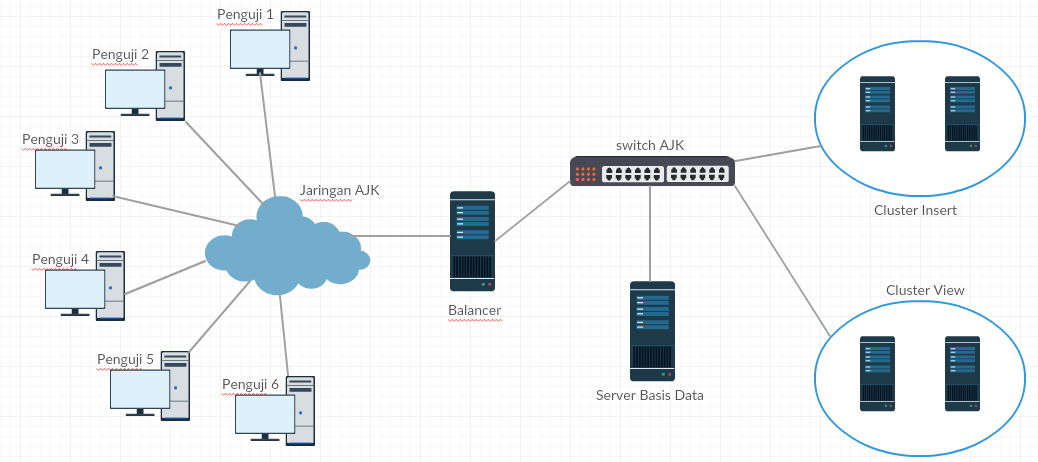
\includegraphics[width=\linewidth]{contoh_img/arsitekturujicoba}
				\caption{Arsitektur Uji Coba}
				\label{gambarArsitekturUjiCoba}
			\end{figure}
			
			Spesifikasi untuk setiap komponen yang digunakan adalah sebagai berikut:
			\begin{itemize}
				\item Balancer:
				\begin{itemize}
					\item Perangkat Keras:
					\begin{itemize}
						\item Processor Intel(R) Core(TM) i3-2120 CPU @ 3.30GHz
						\item RAM 8192 MB
						\item Hard disk 130 GB
					\end{itemize}
					\item Perangkat Lunak:
					\begin{itemize}
						\item Sistem operasi Ubuntu LTS 14.04.03
						\item Nginx 1.4.6
						\item Node JS 4.2.3
						\item MongoDB 3.2.0
						\item PHP 5.5.9
						\item OpenSSH
					\end{itemize}
				\end{itemize}
				\item Worker:
				\begin{itemize}
					\item Worker 1:
					\begin{itemize}
						\item Perangkat Keras:
						\begin{itemize}
							\item Processor Intel(R) Core(TM)2 CPU 4400 @
							2.00GHz
							\item RAM 2048 GB
							\item Hard disk 80 GB
						\end{itemize}
						\item Perangkat Lunak:
						\begin{itemize}
							\item Sistem operasi Ubuntu LTS 14.04.03
							\item Nginx 1.4.6
							\item PHP 5.5.9
							\item OpenSSH
						\end{itemize}
					\end{itemize}
					\item Worker 2:
					\begin{itemize}
						\item Perangkat Keras:
						\begin{itemize}
							\item Processor Intel(R) Core(TM)2 Duo CPU E7200
							@ 2.53GHz
							\item RAM 2048 GB
							\item Hard disk 250 GB
						\end{itemize}
						\item Perangkat Lunak:
						\begin{itemize}
							\item Sistem operasi Ubuntu LTS 14.04.03
							\item Nginx 1.4.6
							\item PHP 5.5.9
							\item OpenSSH
						\end{itemize}
					\end{itemize}
					\item Worker 3 dan 4:
					\begin{itemize}
						\item Perangkat Keras:
						\begin{itemize}
							\item Processor Intel(R) Core(TM) i3-2120 CPU @
							3.30GHz
							\item RAM 4096 GB
							33
							\item Hard disk 500 GB
						\end{itemize}
						\item Perangkat Lunak:
						\begin{itemize}
							\item Sistem operasi Ubuntu LTS 14.04.03
							\item Nginx 1.4.6
							\item PHP 5.5.9
							\item OpenSSH
						\end{itemize}
					\end{itemize}
				\end{itemize}
				\item Server basis data:
				\begin{itemize}
					\item Perangkat Keras:
					\begin{itemize}
						\item Processor Intel(R) Core(TM) i3-2120 CPU @ 3.30GHz
						\item RAM 4096 GB
						\item Hard disk 500 GB
					\end{itemize}
					\item Perangkat Lunak:
					\begin{itemize}
						\item Sistem operasi Ubuntu LTS 14.04.03
						\item MySQL 14.14 Distrib 5.5.44
					\end{itemize}
				\end{itemize}
				\item Komputer Penguji:
				\begin{itemize}
					\item Perangkat Lunak:
					\begin{itemize}
						\item Sistem operasi Windows 7 dan Windows 8.1
						\item Apache Jmeter 2.13
					\end{itemize}
				\end{itemize}
				
			\end{itemize}
			
			Untuk akses ke masing-masing komponen, dibutuh pembagian alamat IP sesuai dengan jaringan AJK yaitu :
			
			\begin{itemize}
				\item Balancer pada 10.151.36.37
				\item Worker 1 pada 10.151.36.21
				\item Worker 2 pada 10.151.36.34
				\item Worker 3 pada 10.151.36.201
				\item Worker 4 pada 10.151.36.203
				\item Server Basis Data pada 10.151.36.205
				\item Penguji pada 10.151.36.24, 10.151.36.25, 10.151.36.26, 10.151.36.27,
				10.151.36.31 dan 10.151.36.32
			\end{itemize}
			
		\section{Skenario Uji Coba}
			Pengujian menggunakan aplikasi berbasis web yang dijalankan pada \textit{worker}. Aplikasi yang digunakan adalah aplikasi Penerimaan Peserta Didik Baru Kota Surabaya tahun 2015. Skenario pengujian dibedakan menjadi 2 bagian yaitu :
			\begin{itemize}
				\item \textbf{Uji Fungsionalitas}. Pengujian ini didasarkan pada fungsionalitas yang disajikan sistem. Sistem sendiri memiliki 3 fitur utama yaitu pembagi beban, kontrol layanan dan halaman admin.
				\item \textbf{Uji Performa}. Pengujian ini untuk menguji ketahanan sistem terhadap sejumlah permintaan yang masuk. Pengujian dilakukan dengan melakukan benchmark pada sistem.
			\end{itemize}
			
			\subsection{Skenario Uji Fungsionalitas}
				Dengan adanya tiga fitur pada balancer, sehingga pengujian akan dilakukan pada tiga fitur secara terpisah.
				\begin{itemize}
					\item \textbf{Pembagi Beban} \\
					Sistem yang berjalan akan memisahkan permintaan yang menuju	ke halaman insert dan halaman view. Pada pengujian ini diharapkan setiap permintaan diarahkan ke klaster yang sesuai. Permintaan dari pengguna dilihat dari URL yang diakses. Kategori URL dan \textit{worker} yang melayani tertera pada Tabel \ref{tabelKategoriURL}.
					
					\begin{longtable}{|p{0.2\textwidth}|p{0.3\textwidth}|p{0.3\textwidth}|} % L = Rata kiri untuk setiap kolom, | = garis batas vertikal.
						
						% Kepala tabel, berulang di setiap halaman
						\caption{Kategori URL dan Klaster Worker} \label{tabelKategoriURL} \\
						\hline
						\textbf{Cookie} & \textbf{Kategori URL} & \textbf{Alamat IP Worker} \\ \hline
						
						\endhead
						\endfoot
						\endlastfoot
						
						% Isi Tabel
						Ada & View & 10.151.36.21 \\ \cline{3-3}
						&& 10.151.36.34 \\ \hline
						Ada & Insert & 10.151.36.201 \\ \cline{3-3}
						&& 10.151.36.203 \\ \hline
						Tidak ada & View, Insert & 10.151.36.201 \\ \hline
						
						
					\end{longtable}
					
					\item \textbf{Kontrol Layanan} \\
					Kontrol Layanan akan mengeluarkan secara sementara \textit{worker} yang sedang tidak aktif dari klasternya. Ketika \textit{worker} sudah kembali pada fase aktif dan siap melayani, kontrol layanan akan kembali memasukkan \textit{worker} ke dalam sistem. Pengujian ini akan memastikan \textit{worker} yang sedang tidak aktif, benar-benar tidak mendapatkan aliran permintaan dari pengguna.
					
					Pengujian dilakukan sebanyak dua kali dengan masing-masing pengujian sebanyak 300 thread. Pada pengujian pertama semua worker akan diaktifkan dan melayani setiap permintaan. Pada pengujian kedua salah satu worker akan dimatikan layanannya tanpa mengubah konfigurasi pada \textit{load balancer}. \textit{Worker} yang tidak melayani tidak akan mengalami penambahan angka \texttt{layani} pada tampilan halaman admin.
					
					
					\item \textbf{Halaman Admin} \\
					Pengujian dilakukan dengan pengaksesan halaman admin yang disediakan sistem dan disesuaikan dengan harapan luaran yang didapatkan. Beberapa hal yang akan diuji berdasarkan pengendali pada halaman admin seperti yang tertera pada Tabel \ref{tabelUjiFungsionalitas}.
				\end{itemize}
				
				\begin{longtable}{|p{0.05\textwidth}|p{0.17\textwidth}|p{0.4\textwidth}|p{0.2\textwidth}|} % L = Rata kiri untuk setiap kolom, | = garis batas vertikal.
					
					% Kepala tabel, berulang di setiap halaman
					\caption{Implementasi Uji Fungsionalitas Halaman Admin} \label{tabelUjiFungsionalitas} \\
					\hline
					\textbf{No} & \textbf{Pengendali} & \textbf{Uji Coba} & \textbf{Hasil Harapan} \\ \hline
					
					\endhead
					\endfoot
					\endlastfoot
					
					% Isi Tabel
					
					1 & /index & Melihat status balancer, IP default, waktu cek & Status balancer (aktif atau tidak), IP worker default tampil, waktu cek tampil \\ \cline{3-4}
					&& Mengaktifkan	balancer & Status balancer aktif dan servis balancer berjalan \\ \cline{3-4}
					&& Mematikan balancer & Status balancer nonaktif dan servis balancer mati \\ \cline{3-4}
					&& Mengganti IP worker default & IP worker berubah dan ditampilkan \\ \cline{3-4}
					&& Mengganti waktu cek & Waktu cek berubah dan ditampilkan \\ \hline
					2 & /cluster & Melihat daftar \textit{worker} pada klaster & Daftar \textit{worker} dalam klaster \\ \cline{3-4}
					&& Menambahkan \textit{worker} ke dalam klaster & Worker dalam klaster bertambah \\ \cline{3-4}
					&& Menghapus \textit{worker} dari klaster & Worker dalam klaster berkurang \\ \hline
					3 & /path & Melihat daftar URL untuk setiap klaster & Daftar URL \\ \cline{3-4}
					&& Menambahkan URL ke dalam klaster & URL dalam klaster bertambah \\ \cline{3-4}
					&& Menghapus URL dari dalam klaster & URL dalam klaster berkurang \\ \hline
					
				\end{longtable}
			
			\subsection{Skenario Uji Performa}
				Pada pengujian ini dilakukan benchmark dengan menggunakan aplikasi berbasis Java yaitu Apache JMeter (). Karena balancer melakukan pemisahan akses, pengujian akan berlangsung berupa insert dan view. Akses insert akan melakukan pendaftaran ke aplikasi PPDB Surabaya 2015 pada jenjang SMA Umum, sedangkan akses view akan menampilkan beberapa halaman pada aplikasi yang sama sekali tidak melakukan insert ke basis data. Apache JMeter akan membuat thread untuk setiap akses ke aplikasi. Pengujian akan berlangsung bertahap mulai dari 300, 600, 900, 1200 dan 1500 thread dalam satu detik. Dari hasil pengujian akan didapatkan waktu respon terhadap permintaan. Waktu ini akan dibandingkan dengan penggunaan arsitektur yang dibangun pada pelaksanaan PPDB Surabaya 2015. Arsitektur sistem PPDB Surabaya 2015 tertera pada Gambar \ref{gambarArsitekturPPDB}.
		
				\begin{figure}[h] % h = pasti berada di bawah teks yang ada di atas
					\centering
					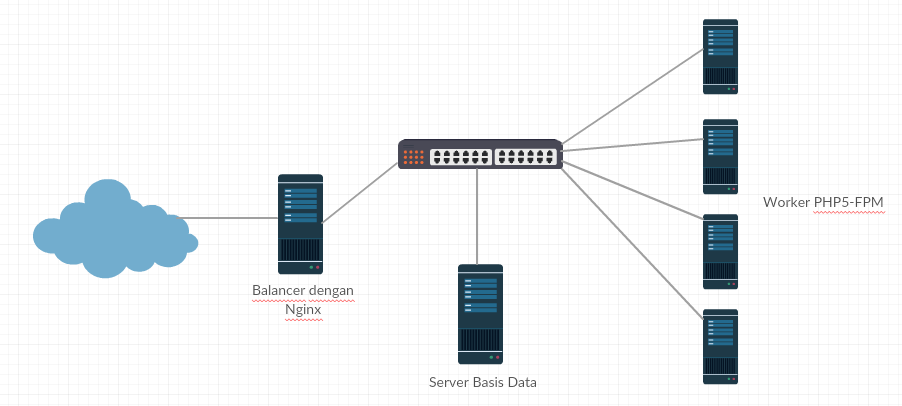
\includegraphics[width=\linewidth]{contoh_img/arsitekturppdb}
					\caption{Arsitektur Jaringan PPDB Surabaya 2015}
					\label{gambarArsitekturPPDB}
				\end{figure}
		
		\section{Hasil Uji Coba dan Evaluasi}
			Berikut dijelaskan hasil uji coba dan evaluasi berdasarkan skenario yang sudah dijelaskan pada bab 5.2.
			
			\subsection{Uji Fungsionalitas}
				Berikut dijelaskan hasil pengujian fungsionalitas pada sistem yang sudah dibangun.
				
				\subsubsection{Pembagi Beban}
					Dilakukan pengujian acak untuk mengakses aplikasi PPDB Surabaya 2015 melalui balancer NodeJS. Hasil pengujian seperti tertera pada Tabel
					
					\begin{longtable}{|p{0.13\textwidth}|p{0.13\textwidth}|p{0.33\textwidth}|p{0.2\textwidth}|p{0.07\textwidth}|} % L = Rata kiri untuk setiap kolom, | = garis batas vertikal.
						
						% Kepala tabel, berulang di setiap halaman
						\caption{Daftar Akses URL dan Worker yang Melayani} \label{tabelBagiBeban} \\
						\hline
						\textbf{Cookie} & \textbf{Kategori} & \textbf{URL} & \textbf{Worker} & \textbf{Hasil}\\ \hline
						
						\endhead
						\endfoot
						\endlastfoot
						
						% Isi Tabel
						kosong & insert & /pendaftaran/pilih\_kk & 10.151.36.201 & OK\\ \hline
						kosong & view & /umum/sambutan & 10.151.36.201 & OK\\ \hline
						ada & view & /umum/ketentuan & 10.151.36.21 & OK\\ \hline
						ada & insert & /pendaftaran & 10.151.36.203 & OK\\ \hline
						ada & view & /umum/subrayon & 10.151.36.21 & OK\\ \hline
						kosong & insert & /pendaftaran/pilih\_kk & 10.151.36.201 & OK\\ \hline
						kosong & view & /umum/sambutan & 10.151.36.201 & OK\\ \hline
						ada & view & /umum/inklusif & 10.151.36.21 & OK\\ \hline
						ada & view & /umum/jadwal & 10.151.36.21 & OK\\ \hline
						ada & view & /umum/ketentuan & 10.151.36.21 & OK\\ \hline
						ada & view & /rekap/lihat/sma/umum & 10.151.36.21 & OK\\ \hline
						ada & insert & /pendaftaran & 10.151.36.201 & OK\\ \hline
						ada & view & /umum/subrayon & 10.151.36.21 & OK\\ \hline
						ada & insert & /pendaftaran/view & 10.151.36.203 & OK\\ \hline
						ada & view & /umum/inklusif & 10.151.36.21 & OK\\ \hline
						kosong & insert & /pendaftaran/pilih\_kk & 10.151.36.201 & OK\\ \hline
						kosong & view & /umum/sambutan & 10.151.36.201 & OK\\ \hline
						ada & view & /umum/jadwal & 10.151.36.21 & OK\\ \hline
						ada & view & /umum/ketentuan & 10.151.36.21 & OK\\ \hline
						ada & view & /rekap/lihat/sma/umum & 10.151.36.21 & OK\\ \hline
						ada & insert & /pendaftaran/submit & 10.151.36.203 & OK\\ \hline
						ada & insert & /pendaftaran & 10.151.36.203 & OK\\ \hline
						ada & view & /umum/subrayon & 10.151.36.21 & OK\\ \hline
						ada & insert & /pendaftaran/view & 10.151.36.201 & OK\\ \hline
						ada & view & /umum/inklusif & 10.151.36.21 & OK\\ \hline
						ada & view & /umum/jadwal & 10.151.36.21 & OK\\ \hline
						ada & view & /rekap/lihat/sma/umum & 10.151.36.21 & OK\\ \hline
						ada & insert & /pendaftaran/submit & 10.151.36.201 & OK\\ \hline
						ada & insert & /pendaftaran/submit & 10.151.36.203 & OK\\ \hline
						ada & insert & /pendaftaran/view & 10.151.36.203 & OK\\ \hline
						ada & insert & /pendaftaran/submit & 10.151.36.201 & OK\\ \hline
						ada & insert & /pendaftaran/submit & 10.151.36.203 & OK\\ \hline
						ada & insert & /pendaftaran/submit & 10.151.36.203 & OK\\ \hline
						ada & insert & /pendaftaran/submit & 10.151.36.203 & OK\\ \hline
						ada & insert & /pendaftaran/submit & 10.151.36.201 & OK\\ \hline
						ada & insert & /pendaftaran/submit & 10.151.36.203 & OK\\ \hline
						ada & insert & /pendaftaran/submit & 10.151.36.203 & OK\\ \hline
						ada & insert & /pendaftaran/submit & 10.151.36.201 & OK\\ \hline
						ada & insert & /pendaftaran/submit & 10.151.36.203 & OK\\ \hline
						ada & insert & /pendaftaran/submit & 10.151.36.201 & OK\\ \hline
						ada & insert & /pendaftaran/submit & 10.151.36.203 & OK\\ \hline
						ada & insert & /pendaftaran/submit & 10.151.36.203 & OK\\ \hline
						ada & insert & /pendaftaran/submit & 10.151.36.201 & OK\\ \hline
						ada & insert & /pendaftaran/submit & 10.151.36.203 & OK\\ \hline
						ada & insert & /pendaftaran/submit & 10.151.36.201 & OK\\ \hline
						ada & insert & /pendaftaran/submit & 10.151.36.203 & OK\\ \hline
						ada & view & /rekap/lihat/sma/umum & 10.151.36.21 & OK\\ \hline
						ada & insert & /pendaftaran/submit & 10.151.36.201 & OK\\ \hline
						ada & insert & /pendaftaran/submit & 10.151.36.203 & OK\\ \hline
						ada & insert & /pendaftaran/submit & 10.151.36.203 & OK\\ \hline
						ada & insert & /pendaftaran/submit & 10.151.36.203 & OK\\ \hline
						ada & view & /rekap/lihat/sma/umum & 10.151.36.21 & OK\\ \hline
						ada & view & /rekap/lihat/sma/umum & 10.151.36.21 & OK\\ \hline
						
						
					\end{longtable}
					
					Sesuai dengan skenario ujicoba yang diberikan pada Tabel \ref{tabelKategoriURL}, hasil ujicoba pada pembagian beban ke klaster yang sesuai dengan kategori 100\% berhasil dilaksanakan. Cookie yang ada tidak ditampilkan untuk memberikan ruang pada penyajian data, karena panjang cookie setiap permintaan akan membuat penyajian data tidak mudah dibaca.
									
				\subsubsection{Kontrol Layanan}
					Sesuai dengan skenario pengujian yang akan dilakukan, pengujian dilakukan sebanyak dua kali. Servis yang dilayani worker untuk dua kali pengujian tertera pada Tabel \ref{tabelKontrolLayanan}.
					
					\begin{longtable}{|p{0.15\textwidth}|p{0.15\textwidth}|p{0.15\textwidth}|p{0.15\textwidth}|p{0.15\textwidth}|} % L = Rata kiri untuk setiap kolom, | = garis batas vertikal.
						
						% Kepala tabel, berulang di setiap halaman
						\caption{Daftar Layani Worker} \label{tabelKontrolLayanan} \\
						\hline
						\textbf{Pengujian} & \textbf{Worker 1} & \textbf{Worker 2} & \textbf{Worker 3} & \textbf{Worker 4}\\ \hline
						
						\endhead
						\endfoot
						\endlastfoot
						
						1 & 75 & 75 & 150 & 149 \\ \hline
						2 & 0 & 150 & 150 & 150 \\ \hline
						
					\end{longtable}
					
					Worker 1 tidak mendapatkan aliran permintaan dari pengguna karena worker 1 dimatikan pada pengujian kedua. Load balancer me-non-aktif-kan fungsi worker 1 sebagai pelayan. Sehingga tidak ada satupun permintaan yang dikirim ke worker 1. Kedua pengujian menghasilkan 100\% sukses.
				
				\subsubsection{Halaman Admin}
					Pengujian dilakukan sesuai dengan skenario ujicoba. Hasil dan evaluasi yang didapatkan dari pengujian halaman admin tertera pada Tabel \ref{tabelUjiFungsionalitasHasil}.
					
					\begin{longtable}{|p{0.05\textwidth}|p{0.17\textwidth}|p{0.35\textwidth}|p{0.25\textwidth}|} % L = Rata kiri untuk setiap kolom, | = garis batas vertikal.
						
						% Kepala tabel, berulang di setiap halaman
						\caption{Uji Fungsionalitas Halaman Admin} \label{tabelUjiFungsionalitasHasil} \\
						\hline
						\textbf{No} & \textbf{Pengendali} & \textbf{Uji Coba} & \textbf{Hasil} \\ \hline
						
						\endhead
						\endfoot
						\endlastfoot
						
						% Isi Tabel
						
						1 & /index & Melihat status balancer, IP default, waktu cek & Sukses - 1190 ms \\ \cline{3-4}
						&& Mengaktifkan	balancer & Sukses - 354 ms \\ \cline{3-4}
						&& Mematikan balancer & Sukses - 372 ms \\ \cline{3-4}
						&& Mengganti IP worker default & Sukses - 17 ms \\ \cline{3-4}
						&& Mengganti waktu cek & Sukses - 16 ms \\ \hline
						2 & /cluster & Melihat daftar \textit{worker} pada klaster & Sukses - 1300 ms \\ \cline{3-4}
						&& Menambahkan \textit{worker} ke dalam klaster & Sukses - 105 ms \\ \cline{3-4}
						&& Menghapus \textit{worker} dari klaster & Sukses - 26 ms \\ \hline
						3 & /path & Melihat daftar URL untuk setiap klaster & Sukses - 1820 ms \\ \cline{3-4}
						&& Menambahkan URL ke dalam klaster & Sukses - 38 ms \\ \cline{3-4}
						&& Menghapus URL dari dalam klaster & Sukses - 48 ms \\ \hline
						
					\end{longtable}
					
			
			\subsection{Uji Performa}
				Seperti yang sudah dijelaskan pada bab 5.2 pengujian performa dilakukan bertahap dengan menggunakan jumlah thread yang bertahap. Beberapa hal yang dibandingkan adalah sebagai berikut:
				
				\subsubsection{Penggunaan CPU dan Memori}
					Pengujian dilakukan hingga jumlah thread mencapai 1500. Hasil pengujian pada dua platform yaitu Nginx dan Node JS tertera pada Gambar \ref{gambarUsage1500}.
					
					\begin{figure}[h] % h = pasti berada di bawah teks yang ada di atas
						\centering
						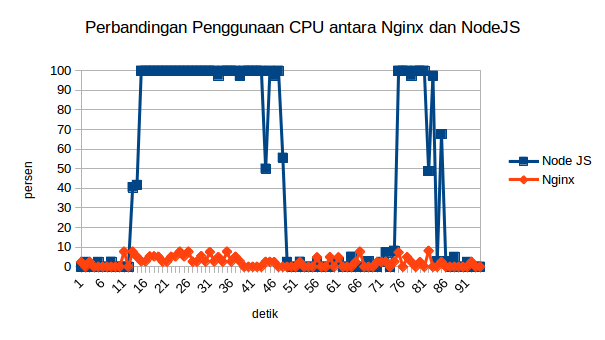
\includegraphics[width=\linewidth]{contoh_img/perbandingan-cpu}
						\caption{Perbandingan Penggunaan CPU pada 1500 thread}
						\label{gambarUsage1500}
					\end{figure}
					
					Rata-rata penggunaan CPU ketika koneksi yang masuk berjumlah 1500 koneksi adalah 100\% untuk NodeJS. Jika dibandingkan dengan penggunaan arsitektur lama pada aplikasi PPDB Surabaya 2015, balancer dengan NodeJS memiliki performas buruk dalam hal penggunaan CPU. Hal ini dikarenakan NodeJS akan membuat sebuah thread untuk setiap koneksi yang masuk ke sistem. Thread ini lah yang menjamin keberlangsungan proses yang berjalan secara asinkronus dapat tetap berjalan.
					
					Sementara untuk penggunaan memori tidak ada perubahan yang signifikan. Ketika menggunakan thread berjumlah 1500 kenaikan penggunaan memori hanya mencapai 20\% saja. Hasil pengujian penggunaan memori tertera pada Gambar \ref{gambarMemoryUsage}.
					
					\begin{figure}[h] % h = pasti berada di bawah teks yang ada di atas
						\centering
						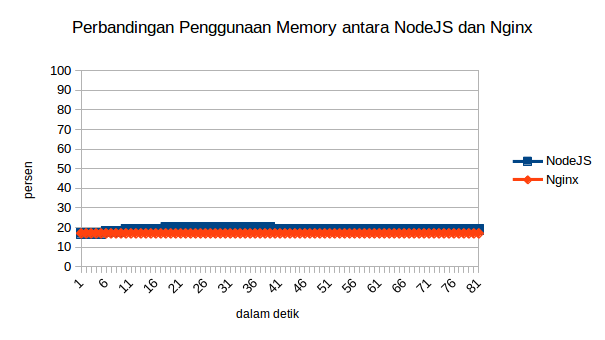
\includegraphics[width=\linewidth]{contoh_img/perbandingan-memori}
						\caption{Penggunaan Memori pada 1500 Thread}
						\label{gambarMemoryUsage}
					\end{figure}
					
					Kedua platform memang tidak menggunakan banyak memori untuk melayani permintaan dari pengguna. Nginx memanfaatkan multi-thread sementara NodeJS menggunakan single-thread. Mekanisme ini akan lebih memakan CPU dibandingkan memori.
				
				\subsubsection{Waktu Respon}
					Pengujian waktu respon dilakukan dengan melakukan insert dan view secara bersamaan ke dalam sistem. Waktu yang digunakan dicatat pada Apache JMeter dan disajikan pada tampilan grafik yang memudahkan untuk dibaca. 
					
					Pengujian dilakukan dengan kombinasi yang berbeda-beda pada setiap klaster. Kombinasi jumlah \textit{worker} dalam klaster untuk pengujian tertera pada Tabel \ref{tabelKombinasi}.
					
					\begin{longtable}{|p{0.3\textwidth}|p{0.3\textwidth}|} % L = Rata kiri untuk setiap kolom, | = garis batas vertikal.
						
						% Kepala tabel, berulang di setiap halaman
						\caption{Kombinasi Jumlah Worker dalam Klaster untuk Uji Coba} \label{tabelKombinasi} \\
						\hline
						\textbf{Klaster Insert} & \textbf{Klaster View} \\ \hline
						
						\endhead
						\endfoot
						\endlastfoot
						
						% Isi Tabel
						1 Worker (2 GB) & 3 Worker \\ \hline
						1 Worker (4 GB) & 3 Worker \\ \hline
						2 Worker (2 GB) & 2 Worker (4 GB) \\ \hline
						2 Worker (4 GB) & 2 Worker (2 GB) \\ \hline
						2 Worker (campur) & 2 Worker (campur) \\ \hline
						3 Worker & 1 Worker (2 GB) \\ \hline
						3 Worker & 1 Worker (4 GB) \\ \hline
						4 Worker & 4 Worker \\ \hline
						
						
					\end{longtable}
					
					Untuk setiap kombinasi dilakukan pengujian dengan jumlah thread dari 300 hingga 1500 thread. Dari semua kombinasi yang dilakukan didapatkan hasil terbaik dengan waktu respon tercepat. Hasil waktu respon terbaik ini dibandingkan dengan hasil pengujian pada arsitektur sistem PPDB Surabaya 2015. Hasil yang didapatkan tertera pada Gambar \ref{gambarPerbandingan}.
					
					Nginx bekerja lebih cepat dibandingkan dengan balancer dengan NodeJS. Pada kenyataannya yang digunakan Nginx adalah 4 worker untuk semua akses, sementara NodeJS membagi worker menjadi klaster tersendiri untuk melayani setiap permintaan. Jika NodeJS menggunakan setiap worker untuk semua akses, waktu respon yang didapatkan jauh lebih lama dibandingkan dengan worker yang dibagi. Hasil pengujiaannya dapat dilihat pada lembar lampiran.
					
					\begin{figure}[h] 
						\centering
						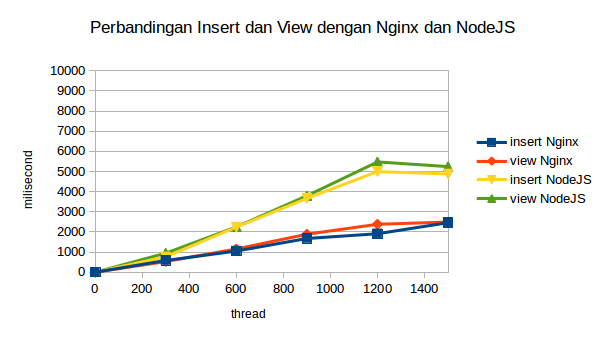
\includegraphics[width=\linewidth]{contoh_img/hasil-perbandingan}
						\caption{Perbandingan Waktu Respon Nginx dan NodeJS}
						\label{gambarPerbandingan}
					\end{figure}
					
				\subsubsection{Permintaan Terlayani}
					Pada percobaan dengan 1500 thread, balancer Node JS dengan 4 \textit{worker} pada klaster insert dan 1 \textit{worker} pada klaster view memberikan ketersediaan layanan lebih baik dibandingan dengan Nginx yang menggunakan 4 \textit{worker} untuk semua aktivitas. Perbedaan ini didapatkan dari hasil benchmark yang kemudian di rata-rata nilai error yang muncul setelah benchmark selesai. Hasil yang didapat
					tertera pada Tabel \ref{tabelGalat}.
					
					\begin{longtable}{|p{0.5\textwidth}|p{0.2\textwidth}|p{0.2\textwidth}|} % L = Rata kiri untuk setiap kolom, | = garis batas vertikal.
						
						% Kepala tabel, berulang di setiap halaman
						\caption{Daftar Nilai Galat pada Akses Halaman} \label{tabelGalat} \\
						\hline
						\textbf{Halaman} & \textbf{NodeJS} & \textbf{Nginx} \\ \hline
						
						\endhead
						\endfoot
						\endlastfoot
						
						% Isi Tabel
						Entry No UASBN & 0,00\% & 21,89\% \\ \hline
						Entry PIN & 0,00\% & 19,89\% \\ \hline
						Inklusif & 0,00\% & 10,83\% \\ \hline
						Jadwal & 0,00\% & 6,83\% \\ \hline
						Ketentuan & 0,00\% & 17,17\% \\ \hline
						Open Pendaftaran & 0,00\% & 9,00\% \\ \hline
						Pendaftaran Dalam Kota & 0,00\% & 22,22\% \\ \hline
						Pilih Sekolah1 & 0,00\% & 18,34\% \\ \hline
						Pilih Sekolah2 & 0,00\% & 17,67\% \\ \hline
						Pilih Sub Rayon & 0,00\% & 19,67\% \\ \hline
						Rekapsmaumum & 0,00\% & 5,50\% \\ \hline
						Sambutan & 0,00\% & 6,67\% \\ \hline
						Selesai & 0,00\% & 16,56\% \\ \hline
						Simpan Permanen & 0,00\% & 16,89\% \\ \hline
						Submit & 0,00\% & 16,89\% \\ \hline
						Subrayon & 0,00\% & 12,17\% \\ \hline
						TOTAL & 0,00\% & 15,60\% \\ \hline
						
					\end{longtable}
				
				\subsubsection{Distribusi Beban}
					Pada pengujian ini dilakukan benchmark dengan total 500 thread dimana 500 thread ini dipisah menjadi dua bagian. Bagian pertama menggunakan \texttt{cookie} yang teracak, dalam artian setiap thread yang berjalan akan menggunakan \texttt{cookie} yang berbeda-beda. Sementara bagian kedua adalah thread yang menggunakan 20 \texttt{cookie} yang sama dan berulang ketika setiap \texttt{cookie} sudah digunakan. Masing-masing bagian akan menjalankan 250 thread. 
					
					Pengujian hanya dilakukan pada salah satu klaster, yaitu klaster view. Pengujian ini tidak dilakukan pada dua klaster dan tidak dibandingkan karena memang beban untuk akses ke halaman informasi dan halaman insert berbeda. Hasil pengujian distribusi beban pada klaster view tertera pada Gambar \ref{gambarDistribusi}.
					
					\begin{figure}[h] 
						\centering
						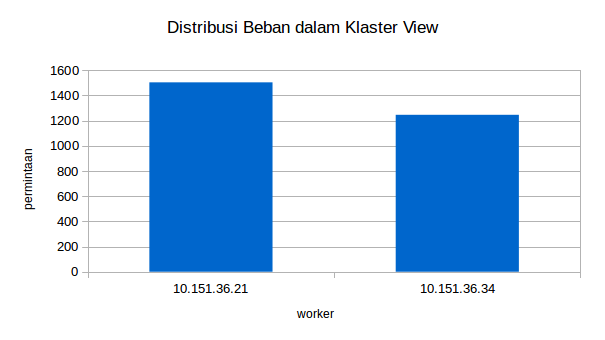
\includegraphics[width=0.8\linewidth]{contoh_img/distribusi}
						\caption{Distribusi Beban pada Klaster View}
						\label{gambarDistribusi}
					\end{figure}
					
					Dengan hasil yang tidak seimbang ini, kemudian dilakukan perubahan mekanisme penyeimbang beban. Awal mekanisme yang digunakan adalah cookie-based dengan pengecekan apakah cookie sudah ada atau belum untuk mendapatkan worker yang akan melayani. Mekanisme ini memaksa pengguna yang sama dilayani oleh worker yang sama. Kemudian mekanisme diganti dengan menggunakan cookie-based dan round robin, dimana cookie tetap diambil namun \textit{worker} yang melayani dipilih dengan menggunakan algoritma round robin.
					
					Mekanisme baru diuji dengan melakukan benchmark yang sama seperti sebelumnya. Dibandingkan dengan mekanisme sebelumnya, hasil yang didapatkan tertera pada Gambar \ref{gambarDistribusiBanding}.
					
					\begin{figure}[h] 
						\centering
						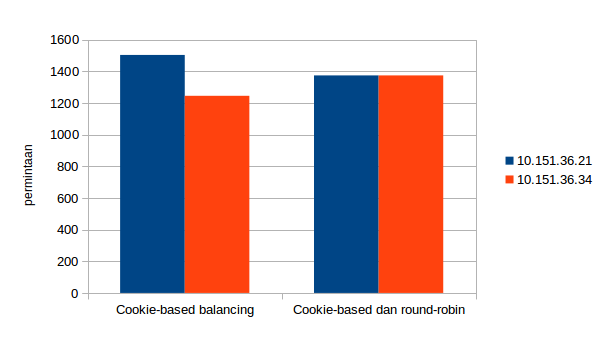
\includegraphics[width=0.8\linewidth]{contoh_img/banding-distribusi}
						\caption{Perbandingan Distribusi Beban Cookie-Based dan Cookie-Based dan Round-Robin}
						\label{gambarDistribusiBanding}
					\end{figure}
					
		\chapter{Penutup}
			Bab ini membahas kesimpulan yang dapat diambil dari tujuan pembuatan sistem dan hubungannya dengan hasil uji coba dan evaluasi yang telah dilakukan. Selain itu, terdapat beberapa saran yang bisa dijadikan acuan untuk melakukan pengembangan dan penelitian lebih lanjut.
			
			\section{Kesimpulan}
				Dari proses perancangan, implementasi dan pengujian terhadap sistem, dapat diambil beberapa kesimpulan berikut:
				\begin{enumerate}
					\item Pembagian beban kerja berdasarkan konten permintaan pengguna dilakukan dengan membaca URL yang diakses pengguna. Pembagian beban kerja berhasil dilakukan dengan pengujian beban kerja yang menghasilkan 100\% sukses. Distribusi beban menjadi tidak merata ketika parameter yang digunakan untuk menjaga pengguna tetap dilayani oleh \textit{worker} yang sama adalah \texttt{cookie}. 
					\item Berdasarkan hasil pengujian didapatkan penggunaan CPU yang meningkat sehingga menyebabkan waktu respon yang makin lama. Hal ini disebabkan NodeJS membuat sebuah thread untuk melayani setiap permintaan baru yang masuk ke sistem.
					\item Kontrol ketersediaan layanan dapat dilakukan dengan melakukan pengecekan servis pada \textit{worker}. Untuk mengeluarkan \textit{worker} dari aktivitas melayani pengguna, tidak dibutuhkan mekanisme untuk merestart sistem. Mekanisme ini menggunakan basis data sebagai dasar balancer untuk meneruskan permintaan.
					\item Dibandingkan dengan sistem yang sudah berjalan sebelumnya, dengan menggunakan Nginx sebagai balancer, NodeJS memberikan hasil penggunaan CPU yang buruk (100\% untuk 1500 thread) sementara Nginx memberikan hasil yang memuaskan (kurang dari 10\% untuk 1500 thread).
				\end{enumerate}
			
			\section{Saran}
				Berikut beberapa saran yang diberikan untuk pengembangan lebih lanjut:
				\begin{itemize}
					\item Mekanisme load balancing yang sudah dirancang perlu ditambah dengan mekanisme pengecekan ketersediaan \textit{worker}. Ketersediaan dapat berupa penggunaan CPU dan memori serta batas \textit{open file} jika memang proses pada \textit{worker} dibatasi \textit{open file}.
					\item Kontrol ketersediaan layanan perlu ditambah parameter untuk memastikan apakah \textit{worker} benar-benar tidak bisa memberikan layanan ke pengguna.
					\item Diperlukan mekanisme lain untuk menjaga pengguna dilayani \textit{worker} yang sama hingga akhir selain menggunakan \texttt{cookie}. Salah satunya dengan round-robin, namun mekanisme ini tidak dapat memastikan worker yang sama melayani pengguna yang sama.
				\end{itemize}
				
		
			\begin{thebibliography}{9}
				\bibitem{paperAlgoritma}
					Saeed Sharifian, Seyed A. Motamedi, Mohammad K. Akbari b,
					\textbf{A content-based load balancing algorithm with admission control for cluster web servers},
					Future Generation Computer Systems,
					vol. 24, pp. 775-787, 2008
				
				\bibitem{webNodeJS}
					Joyent, Inc,
					\textbf{About Node.js}, [Online],
					\url{https://nodejs.org/en/about/},
					diakses tanggal 01 April 2015
					
				\bibitem{useNodeJS}
					S. Tilkov and S. Vinoski,
					\textbf{Node.js: Using JavaScript to Build High-Performance Network Programs},
					IEEE Computer Society Issue,
					vol. 6, pp. 80-83, 2010
					
				\bibitem{clientSideWeb}
					Jeffrey D. Walker, Steven C. Chapra,
					\textbf{A client-side web application for interactive environmental simulation modeling},
					Environmental Modelling \& Software,
					vol. 55, pp. 49-60, 2014
				
				\bibitem{angularJS}
					Google,
					\textbf{Angular JS}, [Online],
					\url{https://angularjs.org/},
					diakses tanggal 07 April 2015
				
				\bibitem{selfDescription}
					Ming Zhang, Jing Zhang, Wei Zheng, Feiran Hu, Ge Zhuang,
					\textbf{A self-description data framework for Tokamak control system design},
					Fusion Engineering and Design,
					p. 5, 2015
				
				\bibitem{mongoDB}
					MongoDB, Inc,
					\textbf{MongoDB}, [Online],
					\url{https://www.mongodb.org/},
					diakses tanggal 08 April 2015
					
				\bibitem{JMeter}
					Apache Software Foundation,
					\textbf{Apache JMeter}, [Online],
					\url{http://jmeter.apache.org/},
					diakses tanggal 08 April 2015
				
				\bibitem{quoraNginx}
					Quora,
					\textbf{Why is nginx so efficient?}, [Online],
					\url{https://www.quora.com/Why-is-nginx-so-efficient},
					diakses tanggal 03 Januari 2016
				
				\bibitem{aosaNginx}
					AOSABook,
					\textbf{nginx}, [Online],
					\url{http://www.aosabook.org/en/nginx.html},
					diakses tanggal 03 Januari 2016
			\end{thebibliography}

\renewcommand\chaptername{LAMPIRAN}
\appendix % Halaman lampiran, dengan judul LAMPIRAN X
	\chapter{Instalasi Perangkat Lunak}
		\section{Instalasi Node JS}
			Ada banyak cara untuk menginstall NodeJS ke dalam komputer, salah satunya melalui kode sumber yang dapat diunduh pada halaman \texttt{https://nodejs.org/en/download/}. Setelah diunduh berkas perlu diekstrak untuk melanjutkan instalasi. Di dalam folder hasil ekstraksi, terdapat berkas \texttt{README.md} yang berisi langkah untuk menginstall NodeJS ke komputer. Semua langkah dilakukan melalui \textit{command line} dan langkah installasinya adalah sebagai berikut
			
			\begin{itemize}
				\item Pindah ke folder dimana Node JS di ekstrak dengan perintah \texttt{cd \{\$pathdownload\}/node-v4.2.3/}.
				\item Di dalam folder jalankan perintah berikut secara berurutan \texttt{./configure}, \texttt{make}, \texttt{make install}.
				\item Jika terdapat pesan \textit{error} mengenai beberapa pustaka yang belum terinstall sebelumnya, jalankan perintah \texttt{sudo apt-get install -f}.
				\item Semua perintah dilakukan pada hak akses \textit{root}.
			\end{itemize}
			
			Untuk memastikan bahwa Node JS sudah berjalan dan siap digunakan, dijalankan perintah dan dihasilkan output seperti pada Gambar \ref{gambarCekNodeJS}.
			
			\begin{figure}[h] % h = pasti berada di bawah teks yang ada di atas
				\centering
				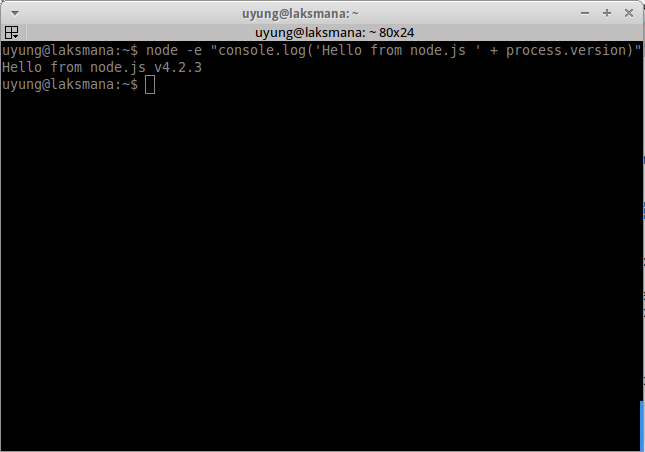
\includegraphics[width=\linewidth]{contoh_img/ceknodejs}
				\caption{Contoh Node JS Siap Digunakan}
				\label{gambarCekNodeJS}
			\end{figure}
		
		\section{Installasi MongoDB}
			MongoDB menyediakan repositori tersendiri untuk mengunduh MongoDB. Setelah terkoneksi dengan repositori yang dimiliki MongoDB, instalasi dapat berlanjut dengan menggunakan perintah \texttt{apt-get}. Berikut ini langkah-langkah instalasi MongoDB.			
			
			\begin{itemize}
				\item Tambahkan \textit{public key} yang digunakan untuk manajemen paket pada sistem operasi dengan perintah \texttt{sudo apt-key adv --keyserver hkp://keyserver.ubuntu.com:80 --recv 7F0CEB10}.
				\item Buat file repositori untuk MongoDB pada sistem komputer dengan perintah \texttt{echo "deb http://repo.mongodb.org/apt/ubuntu trusty/mongodb-org/3.0 multiverse" | sudo tee /etc/apt/sources.list.d/mongodb-org-3.0.list}. Perintah ini disesuaikan dengan distro Linux yang digunakan.
				\item Perbaharui basis data manajemen paket dengan perintah \texttt{sudo apt-get update}.
				\item Install MongoDB ke komputer dengan perintah \texttt{sudo apt-get install -y mongodb-org}.
				\item Setelah instalasi selesai jalankan MongoDB dengan perintah \texttt{sudo service mongod start}.
				\item MongoDB siap digunakan dengan tampilan pada Gambar \ref{gambarCekMongoDB}.								
			\end{itemize}
			
			\begin{figure}[h] % h = pasti berada di bawah teks yang ada di atas
				\centering
				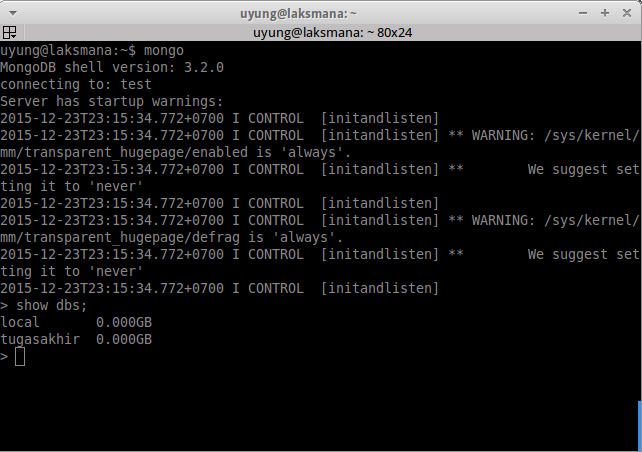
\includegraphics[width=0.8\linewidth]{contoh_img/cekmongodb}
				\caption{Contoh MongoDB dan Daftar Database}
				\label{gambarCekMongoDB}
			\end{figure}
	
	\chapter{Kode Sumber}
		\section{Load Balancer}
			\begin{lstlisting}[frame=single,tabsize=2,breaklines,caption={Kode Sumber Lengkap Load Balancer},label=loadBalancer]	
var http = require('http'),
httpProxy = require('http-proxy'),
proxy = httpProxy.createProxyServer({}),
url = require('url'),
mongoose = require('mongoose');

var clusterview_model = require('./model/clusterview_model')
var clusterinsert_model = require('./model/clusterinsert_model')
var aktivitas_model = require('./model/aktivitas_model')
var path_model = require('./model/path_model')
var setting_model = require('./model/setting_model')

mongoose.connect('mongodb://127.0.0.1/tugasakhir');

http.createServer(function(req, res) {

	var cookie = req.headers.cookie;
	var pengguna;
	if (!cookie) cookie='kosong';
	var awal = cookie.indexOf('csrf_cookie_name');
	var akhir = cookie.indexOf(';', awal)
	if (akhir > awal) {
		pengguna = cookie.substring(awal, akhir)
	}
	else {
		pengguna = cookie.substring(awal, cookie.length)
	}
	
	var fullpath = url.parse(req.url).pathname;
	var pathname = url.parse(req.url).pathname.split("/");
	
	var petugas;
				
	if (pathname[1] == '') {pathname[1]='home'}
	
	path_model.path.findOne({path: pathname[1]}, 'aksi', function(err, result){
		if (err) return handleError(err);
		console.log(result.aksi)
		if (cookie=='kosong') {
			setting_model.setting.findOne({setting:"default"}, 'pakehuruf', function(error, resul){
				if (error) console.log(error)				
				petugas = resul.pakehuruf
				console.log(pengguna,";",result.aksi,";",fullpath,";",petugas)
				proxy.web(req,res,{target : 'http://'+petugas},function(ee,aa){
					console.log("ini error juga", ee)
				});
			})
		}
		else {
			var cari = {cookie: pengguna, aksi: result.aksi}
			aktivitas_model.findAktivitas(cari, function(erro, resu){				
				if (erro) return console.log("kesalahan")
				if (!resu) {
					//dapatkan server yang dapat digunakan
					if (result.aksi == 'view') {
						clusterview_model.findOneClusterView(function(salah, hasil){
							if (salah) return console.log(salah)
							petugas = hasil.ip;
							clusterview_model.updateLayani(hasil.ip, function(wa, we){
								if (wa) return console.log(wa)
								console.log(we);
							})
	
							//tambah pengguna baru ke dalam basis data
							var kumpul = {cookie: pengguna, ip: petugas, aksi: result.aksi}
							aktivitas_model.tambahAktivitas(kumpul,function(errr, ress){
								if (errr) return handleError(errr)
								proxy.web(req, res, {target : 'http://'+petugas},function(ee,aa){
									if(ee) console.log(ee)
								});
							})
						})
					}
					else {
						clusterinsert_model.findOneClusterInsert(function(salah, hasil){
							if (salah) return console.log(salah)
							petugas = hasil.ip;
							clusterinsert_model.updateLayani(hasil.ip, function(wa, we){
								if (wa) return console.log(wa)
								console.log(we);
							})
	
							//tambah pengguna baru ke dalam basis data
							var kumpul = {cookie: pengguna, ip: petugas, aksi: result.aksi}
							aktivitas_model.tambahAktivitas(kumpul,function(errr, ress){
								if (errr) return handleError(errr)
								proxy.web(req, res, {target : 'http://'+petugas}, function(ee,aa){
									if(ee) console.log(ee)
								});
							})
						})
					}
				}
				else {		
					proxy.web(req, res, {target : 'http://'+resu.ip}, function(ee, aa){
					if(ee) console.log("di sini error", ee)
					})
				}
			});
		}
	});
	
}).listen(80, function() {
	console.log('proxy listening on port 80');
});
			
			
			
			\end{lstlisting}
		
		\section{Aktivitas Model}
			\begin{lstlisting}[frame=single,tabsize=2,breaklines,caption={Aktivitas Model untuk Koleksi Aktivitas},label=aktivitasModel]	
var mongoose = require('mongoose');

var aktivitasSchema = new mongoose.Schema({
	cookie: String,
	ip: String,
	aksi: String
},{
	collection : 'aktivitas'
})

var aktivitas = mongoose.model('aktivitas', aktivitasSchema);

exports.aktivitas = aktivitas;

exports.findAktivitas = function(data, callback) {
	aktivitas.findOne({cookie: data.cookie, aksi: data.aksi}, 'aksi ip', function(err, resultIP){
		if(err) console.log(err)
		if(resultIP == null) {
			callback(err, null)
		}
		else {
			callback(err, resultIP)
		}
	})
}

exports.tambahAktivitas = function(data, callback){
	aktivitas.create({cookie: data.cookie, ip: data.ip, aksi: data.aksi},function(errr, ress){
		if (errr) return handleError(errr)
		callback(errr,ress)
	})
}
			
			\end{lstlisting}

		\section{ClusterInsert Model}
			\begin{lstlisting}[frame=single,tabsize=2,breaklines,caption={ClusterInsert Model untuk Koleksi ClusterInsert},label=clusterInsertModel]	
var mongoose = require('mongoose');

var clusterInsertSchema = new mongoose.Schema({
	ip : String,
	online : Boolean,
	layani : Number
},{
	collection : 'clusterInsert'
})

var clusterInsert = mongoose.model('clusterInsert', clusterInsertSchema);

exports.clusterInsert = clusterInsert;

exports.findClusterInsert = function(ip, callback) {
	clusterInsert.findOne({ip: ip}, function(err, resultIP){
		if(err) console.log(err)
		if(resultIP == null) {
			callback(new Error("IP tidak ada"))
		}
		else {
			callback(err, resultIP)
		}
	})
}

exports.findOneClusterInsert = function(callback) {
	clusterInsert.findOne({'online': 1}, 'ip online layani', {sort:{'layani':1},limit:1}, function(err, resultIP){
		if(err) console.log(err)
		if(resultIP == null) {
			callback(err, null)
		}
		else {
			callback(err, resultIP)
		}
	})
}

exports.updateLayani = function(ip, callback) {
	clusterInsert.findOneAndUpdate({ip: ip}, {$inc : {layani: 1}}, function(err, result){
		if (err) return console.log(err)
		callback(err, "sudah ditambahkan")
	})
}

exports.tambahClusterInsert = function(ip, callback){
	exports.findClusterInsert(ip, function(err, resu){
		if(resu == null) {
			var newIP = new clusterInsert({ip: ip, online: 1, layani: 0})
			newIP.save(function(errr){
				callback(errr,newIP)
			})
		} else {
			callback(new Error("IP sudah ada"))
		}
	})
}

exports.hapusClusterInsert = function(ip, callback){
	clusterInsert.findOneAndRemove({ip: ip}, function(err, result){
		if (err) console.log(err)
		callback(err, result)
	})
}
			
			\end{lstlisting}
		
		\section{ClusterView Model}
			\begin{lstlisting}[frame=single,tabsize=2,breaklines,caption={ClusterView Model untuk Koleksi ClusterView},label=clusterViewModel]	
var mongoose = require('mongoose');

var clusterViewSchema = new mongoose.Schema({
	ip : String,
	online : Boolean,
	layani : Number
},{
	collection : 'clusterView'
})

var clusterView = mongoose.model('clusterView', clusterViewSchema);

exports.clusterView = clusterView;

exports.findClusterView = function(ip, callback) {
	clusterView.findOne({ip: ip}, function(err, resultIP){
		if(err) console.log(err)
		if(resultIP == null) {
			callback(new Error("IP tidak ada"))
		}
		else {
			callback(err, resultIP)
		}
	})
}

exports.findOneClusterView = function(callback) {
	clusterView.findOne({'online': 1}, 'ip online layani', {sort:{'layani':1},limit:1}, function(err, resultIP){
		if(err) console.log(err)
		if(resultIP == null) {
			callback(err, null)
		}
		else {
			callback(err, resultIP)
		}
	})
}

exports.updateLayani = function(ip, callback) {
	clusterView.findOneAndUpdate({ip: ip}, {$inc : {layani: 1}}, function(err, result){
		if (err) return console.log(err)
		callback(err, "sudah ditambahkan")
	})
}

exports.tambahClusterView = function(ip, callback){
	exports.findClusterView(ip, function(err, resu){
		if(resu == null) {
			var newIP = new clusterView({ip: ip, online: 1, layani: 0})
			newIP.save(function(errr){
				callback(errr,newIP)
			})
		} else {
			callback(new Error("IP sudah ada"))
		}
	})
}

exports.hapusClusterView = function(ip, callback){
	clusterView.findOneAndRemove({ip: ip}, function(err, result){
	if (err) console.log(err)
	callback(err, result)
	})
}
			
			\end{lstlisting}

		\section{Path Model}
			\begin{lstlisting}[frame=single,tabsize=2,breaklines,caption={Path Model untuk Koleksi URL},label=pathModel]	
var mongoose = require('mongoose');

var pathSchema = new mongoose.Schema({
	path: String,
	aksi: String
},{
	collection : 'path'
})

var path = mongoose.model('path', pathSchema);

exports.path = path;

exports.simpanPathBaru = function(data, callback){
	var newPath = new pathI({path: data.path, aksi: data.aksi})
	newPath.save(function(errr){
		callback(errr,newPath)
	})
}

exports.hapusPath = function(path, callback){
	pathI.findOneAndRemove({path: path}, function(err, result){
		if (err) console.log(err)
		callback(err, result)
	})
}

			
			\end{lstlisting}
		
		\section{Setting Model}
			\begin{lstlisting}[frame=single,tabsize=2,breaklines,caption={Setting Model untuk Koleksi Setting},label=settingModel]	
var mongoose = require('mongoose');

var pathSchema = new mongoose.Schema({
	setting: String,
	pakeangka: Number,
	pakehuruf: String
},{
	collection : 'setting'
})

var settingBalancer = mongoose.model('setting', pathSchema);

exports.setting = settingBalancer;

exports.ubahSettingIP = function(data, callback){
	settingBalancer.findOneAndUpdate({setting: data.setting},{$set : {pakehuruf: data.ip}},function(err, result){
		if (err) console.log(err)
		callback(err, result)
	})
}

exports.ubahSettingWaktu = function(data, callback){
	settingBalancer.findOneAndUpdate({setting: data.setting},{$set : {pakeangka: data.angka}},function(err, result){
		if (err) console.log(err)
		callback(err, result)
	})
}
			
			\end{lstlisting}
	
	\chapter{Grafik Uji Coba dengan berbagai Kombinasi}
		\begin{figure}[h] % h = pasti berada di bawah teks yang ada di atas
			\centering
			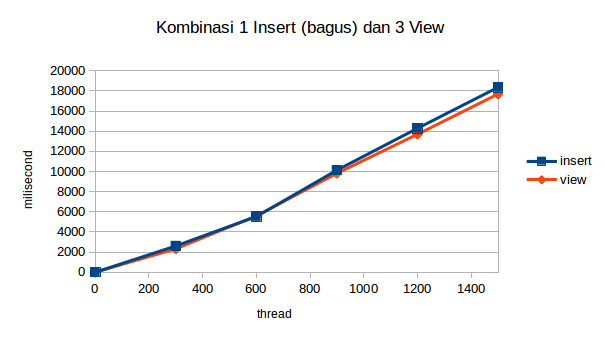
\includegraphics[width=0.85\linewidth]{contoh_img/hasil/1-3-bagus}
			\caption{Kombinasi 1 Insert (bagus) dan 3 View}
			\label{gambar1-3bagus}
		\end{figure}
		
		\begin{figure}[h] % h = pasti berada di bawah teks yang ada di atas
			\centering
			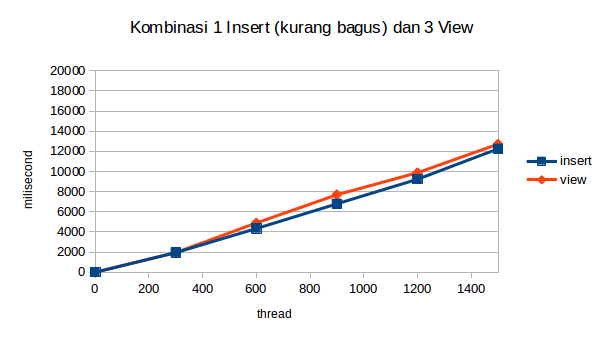
\includegraphics[width=0.85\linewidth]{contoh_img/hasil/1-3-jelek}
			\caption{Kombinasi 1 Insert (jelek) dan 3 View}
			\label{gambar1-3jelek}
		\end{figure}
		
		\begin{figure}[h] % h = pasti berada di bawah teks yang ada di atas
			\centering
			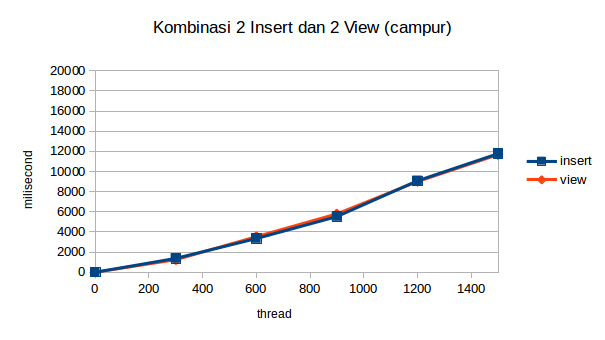
\includegraphics[width=0.85\linewidth]{contoh_img/hasil/2-2-campur}
			\caption{Kombinasi 2 Insert dan 2 View (campur)}
			\label{gambar2-2campur}
		\end{figure}
		
		\begin{figure}[h] % h = pasti berada di bawah teks yang ada di atas
			\centering
			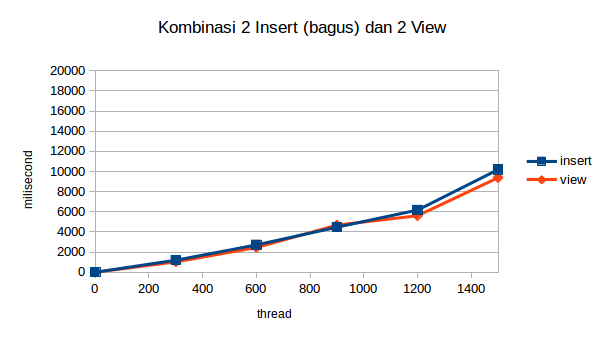
\includegraphics[width=0.85\linewidth]{contoh_img/hasil/2-2-ibagus}
			\caption{Kombinasi 2 Insert (bagus) dan 2 View}
			\label{gambar2-2ibagus}
		\end{figure}
		
		\begin{figure}[h] % h = pasti berada di bawah teks yang ada di atas
			\centering
			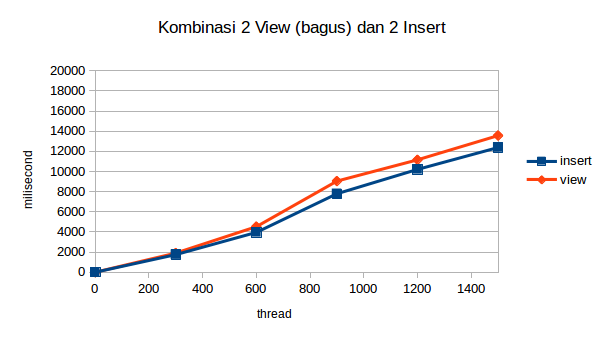
\includegraphics[width=0.85\linewidth]{contoh_img/hasil/2-2-vbagus}
			\caption{Kombinasi 2 View (bagus) dan 2 Insert}
			\label{gambar2-2vbagus}
		\end{figure}
		
		\begin{figure}[h] % h = pasti berada di bawah teks yang ada di atas
			\centering
			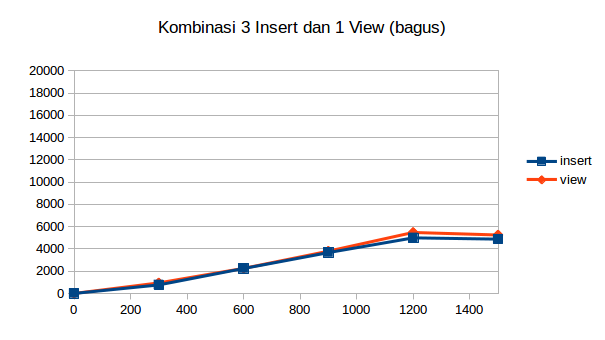
\includegraphics[width=0.85\linewidth]{contoh_img/hasil/3-1-bagus}
			\caption{Kombinasi 3 Insert dan 1 View (bagus)}
			\label{gambar3-1bagus}
		\end{figure}
		
		\begin{figure}[t] % h = pasti berada di bawah teks yang ada di atas
			\centering
			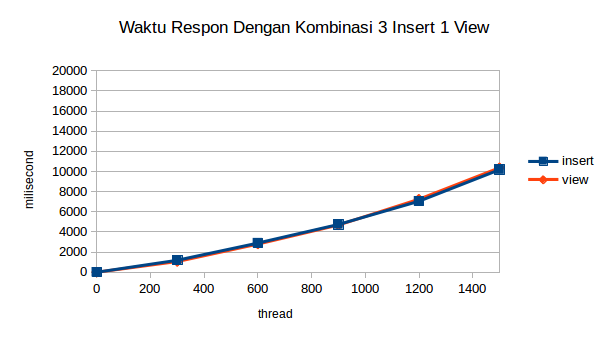
\includegraphics[width=0.85\linewidth]{contoh_img/hasil/3-1-jelek}
			\caption{Kombinasi 3 Insert dan 1 View (jelek)}
			\label{gambar3-1jelek}
		\end{figure}
		

\backmatter % Lampiran tanpa judul LAMPIRAN X, biasanya untuk BIODATA PENULIS
	\chapter{BIODATA PENULIS}
		\begin{wrapfigure}{l}{0.3\textwidth}
			\includegraphics[width=0.29\textwidth]{img/uyung}
		\end{wrapfigure}
		
		\textbf{Bahrul Halimi}, seharusnya memiliki panggilan Rurul, namun karena hal lain menjadi memiliki panggilan Uyung. Pada 20 November 1993 lahir di Pati, Jawa Tengah, kota kecil yang mulai terkenal dengan bisnis karaoke. 17 tahun tidak meninggalkan Pati dan akhirnya memutuskan untuk melanjutkan studi di Institut Teknologi Sepuluh Nopember Surabaya. Penulis mulai akrab dengan dunia komputer pada tingkat pendidikan Sekolah Dasar (SD), namun karena biaya teknologi yang dipelajari tidak sesuai dengan perkembangan pada saat itu. Aktif di dunia koding pada tingkat pendidikan Sekolah Menengah Atas (SMA) dengan mengikuti Olimpiade Komputer, namun tidak pernah lolos pada tingkat provinsi. Hingga buku ini dikeluarkan, penulis masih mendalami ilmu di bidang jaringan pada sisi infrastruktur. Penulis dapat dihubungi melalui surel \texttt{31uyung10@gmail.com}.
\end{document}
